\chapter{Технологическая часть}

В данном разделе происходит выбор средств 
реализации базы данных и приложения, 
листинги кода, а так же будет показан интерфейс программы.


\section{Выбор системы управления базой данных}

В аналитическом разделе была выбрана реляционная 
система управления, наиболее распространнеными представителями
данной системы являются: 
Microsoft SQL, PostgreSQL, Oracle, а также MySQL~\cite{diffdb}. 

Выберем следующие критерии для сравнения выбранных систем:
\begin{enumerate}
    \item[1)] возможность бесплатного использования;
    \item[2)] опыт работы с данной системой;
    \item[3)] наличие подробной документации. 
\end{enumerate}

Сравнение указанных систем управления базой данных(СУБД)
представлены в таблице \ref{tab:diff}:

\begin{table}[!ht]
    \centering
    \caption{\label{tab:diff} Сравнение СУБД по указаным критериям}
    \begin{tabular}{|l|l|l|l|l|}
    \hline
        СУБД & Microsoft SQL & PostgreSQL & Oracle & MySQL \\ \hline
        1 & - & + & - & +  \\ \hline
        2 & - & + & - & -  \\ \hline
        3 & + & + & + & +  \\ \hline
    \end{tabular}
\end{table}

По результатам сравнения для реляционной базы данных была выбрана PostgreSQL, так как это 
единственная система, которая удовлетворяет всем критериям.

\section{Выбор средств реализации}

Реализация части приложения,
которая обеспечивает доступ к базе данных, 
была выполнена с использованием языка программирования GoLang~\cite{golang}. 
Данный выбор обусловлен следующими причинами:

\begin{itemize}
    \item сборщик мусора, который позволяет автоматически
    освобождать память;
    \item статическая типизация, которая помогает 
    обнаруживать ошибки на этапе компиляции;
    \item встроенная поддержка параллельных вычислений, что
    позволяет делать разработку многопоточной.
\end{itemize}

Графический интерфейс был разработан с использованием HTML~\cite{html} и CSS~\cite{css},
так же был выбран язык JavaScript~\cite{jsLang} для 
обработки событий и динамического обновления элементов.

Причина выбора данных средств заключается в следующем:
\begin{itemize}
    \item HTML и CSS поддерживаются всеми основными веб-браузерами, 
    что гарантирует доступность содержимого на различных устройствах;
    \item опыт работы с HTML и CSS;
    \item JS имеет возможность получать доступ к структуре HTML-документа, 
    что позволяет манипулировать элементами, стилями, атрибутами и событиями.
\end{itemize}

\section{Выбор среды разрабоки}

В качестве среды разработки был выбран Visual Studio Code~\cite{vscode}. Данный выбор обусловлен
следующими причинами:
\begin{itemize}
    \item бесплатный доступ;
    \item поддержка выбранных языков;
    \item опыт работы в данной среде.
\end{itemize}

\section{Архитектура приложения}

Для разрабатываемого приложения была выбрана чистая архитектура~\cite{cleanArch}, то есть приложение будет 
состоять из трех слоев: графический интерфейс, бизнес-логика, доступ к данным.

Данное разделение имеет следующие преимущества:
\begin{itemize}
    \item приложение не зависит от используемых библиотек и фреймворков;
    \item удобство тестирования;
    \item возможность использования различных баз данных, так как
    бизнес-логика не зависит напрямую от используемой базы данных;
\end{itemize}

\section{Реализация ролевой модели}
Ранее были определены 3 роли: гость (неавторизованный пользователь), 
владелец дома, а также участник дома. 
В приложении Б\ref{lst:list2.sql} -- Б\ref{lst:list4.sql} представлено создание данных ролей.

\section{Реализация функции}

Функция, осуществляющая обновление текущего статуса 
устройства в зависимости от его состояние представлена 
в приложении~А\ref{lst:list1.sql}. Следует отметить, что если 
устройство работает и какой-то другой участник дома 
захочет его запустить, то фукнция вернет ошибку.  

\section{Тестирование}

Чтобы обеспечить автоматизацию тестирования
использовался пакет testcontainers~\cite{testcontainers}, который
автоматически поднимает контейнеры. Для создания таблиц 
и ограничений к ним в тестируемой базе данных, а так же
для заполнения созданных таблиц использовался пакет goose~\cite{goose}, 
необходимый для использования миграций.

Во время проведения тестов в базе данных содержалась 
следующая информация:

\begin{enumerate}
    \item устройство dev1 с статусом <<Inactive>>;
    \item устройство dev2 с статусом <<Inactive>>;
\end{enumerate}

В таблице \ref{tab:tests} приведены тесты, 
которые использовались для проверки правильности 
работы функции для изменения текущего статуса устройства.

\begin{table}[H]
    \centering
    \caption{\label{tab:tests} Тесты, используемые для проверки правильности 
    работы функции для изменения текущего статуса устройства.}
    \begin{tabular}{|l|l|l|l|l|l|}
    \hline
        Текущее & Новое  & ID & Переданный ID & Ожидаемый & Ответ \\
        состояние & состояние & устройства &  & ответ &  \\ \hline
        inactive & inactive & 1 & 1 & -3 & -3 \\ \hline
        inactive & inactive & 2 & 2 & -3 & -3 \\ \hline
        inactive & active & 2 & 2 & 0 & 0 \\ \hline
        inactive & active & 1 & 1 & 0 & 0 \\ \hline
        active & active & 2 & 2 & -2 & -2 \\ \hline
        active & inactive & 1 & 1 & 0 & 0 \\ \hline
        active & inactive & 2 & 2 & 0 & 0 \\ \hline
    \end{tabular}
\end{table}

Также были проведены тесты для других запросов к базе данных, результат которых представлен 
в приложении В\ref{img:test1} -- В\ref{img:test2}.

\section{Графический интерфейс}

Независимо от роли пользователь попадает на страницу c авторизацией \ref{img:auth}, где ему предоставляется возможность 
войти в личный аккаунт с помощью пароля и почты или зарегистрироваться в системе, также пользователь может восстановить пароль.

\begin{figure}[H]
    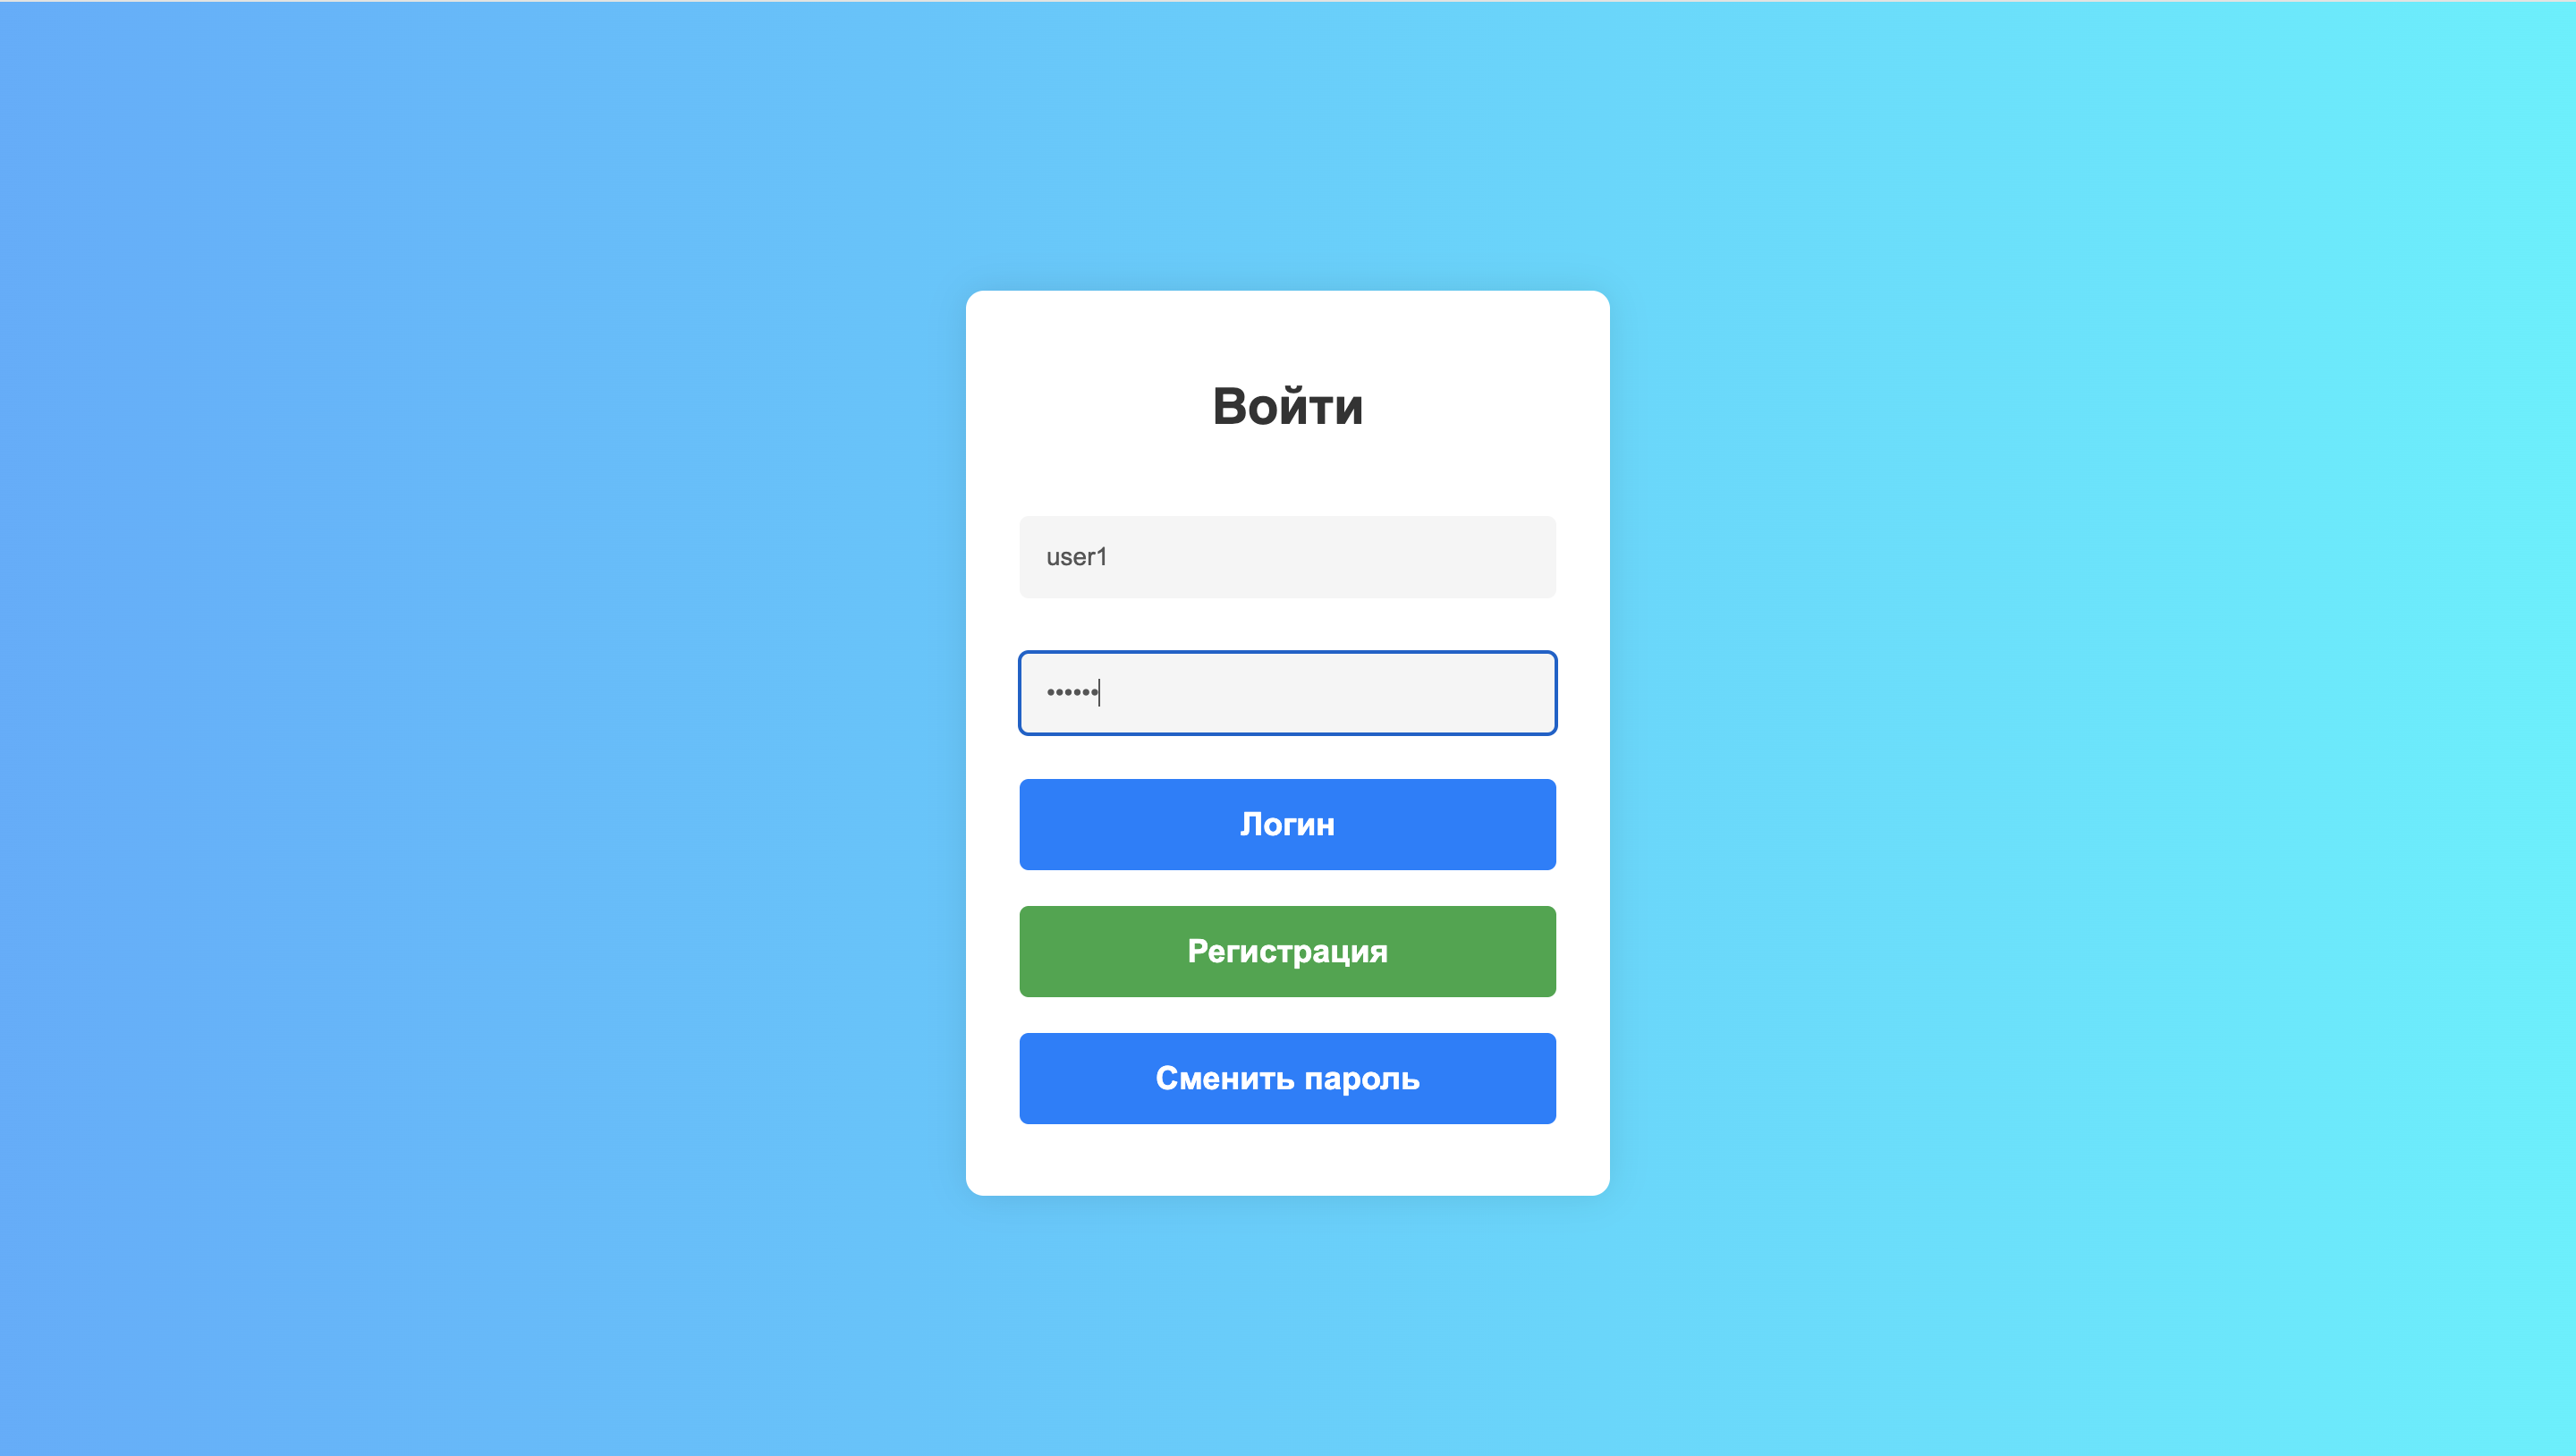
\includegraphics[width=1\linewidth]{img/auth.png}
    \caption{\label{img:auth} Страница для авторизации пользователя}
\end{figure}
\noindent

На странице регистрации пользователь может содать аккаунт, введя логин, пароль и почту \ref{img:reg}.
\begin{figure}[H]
    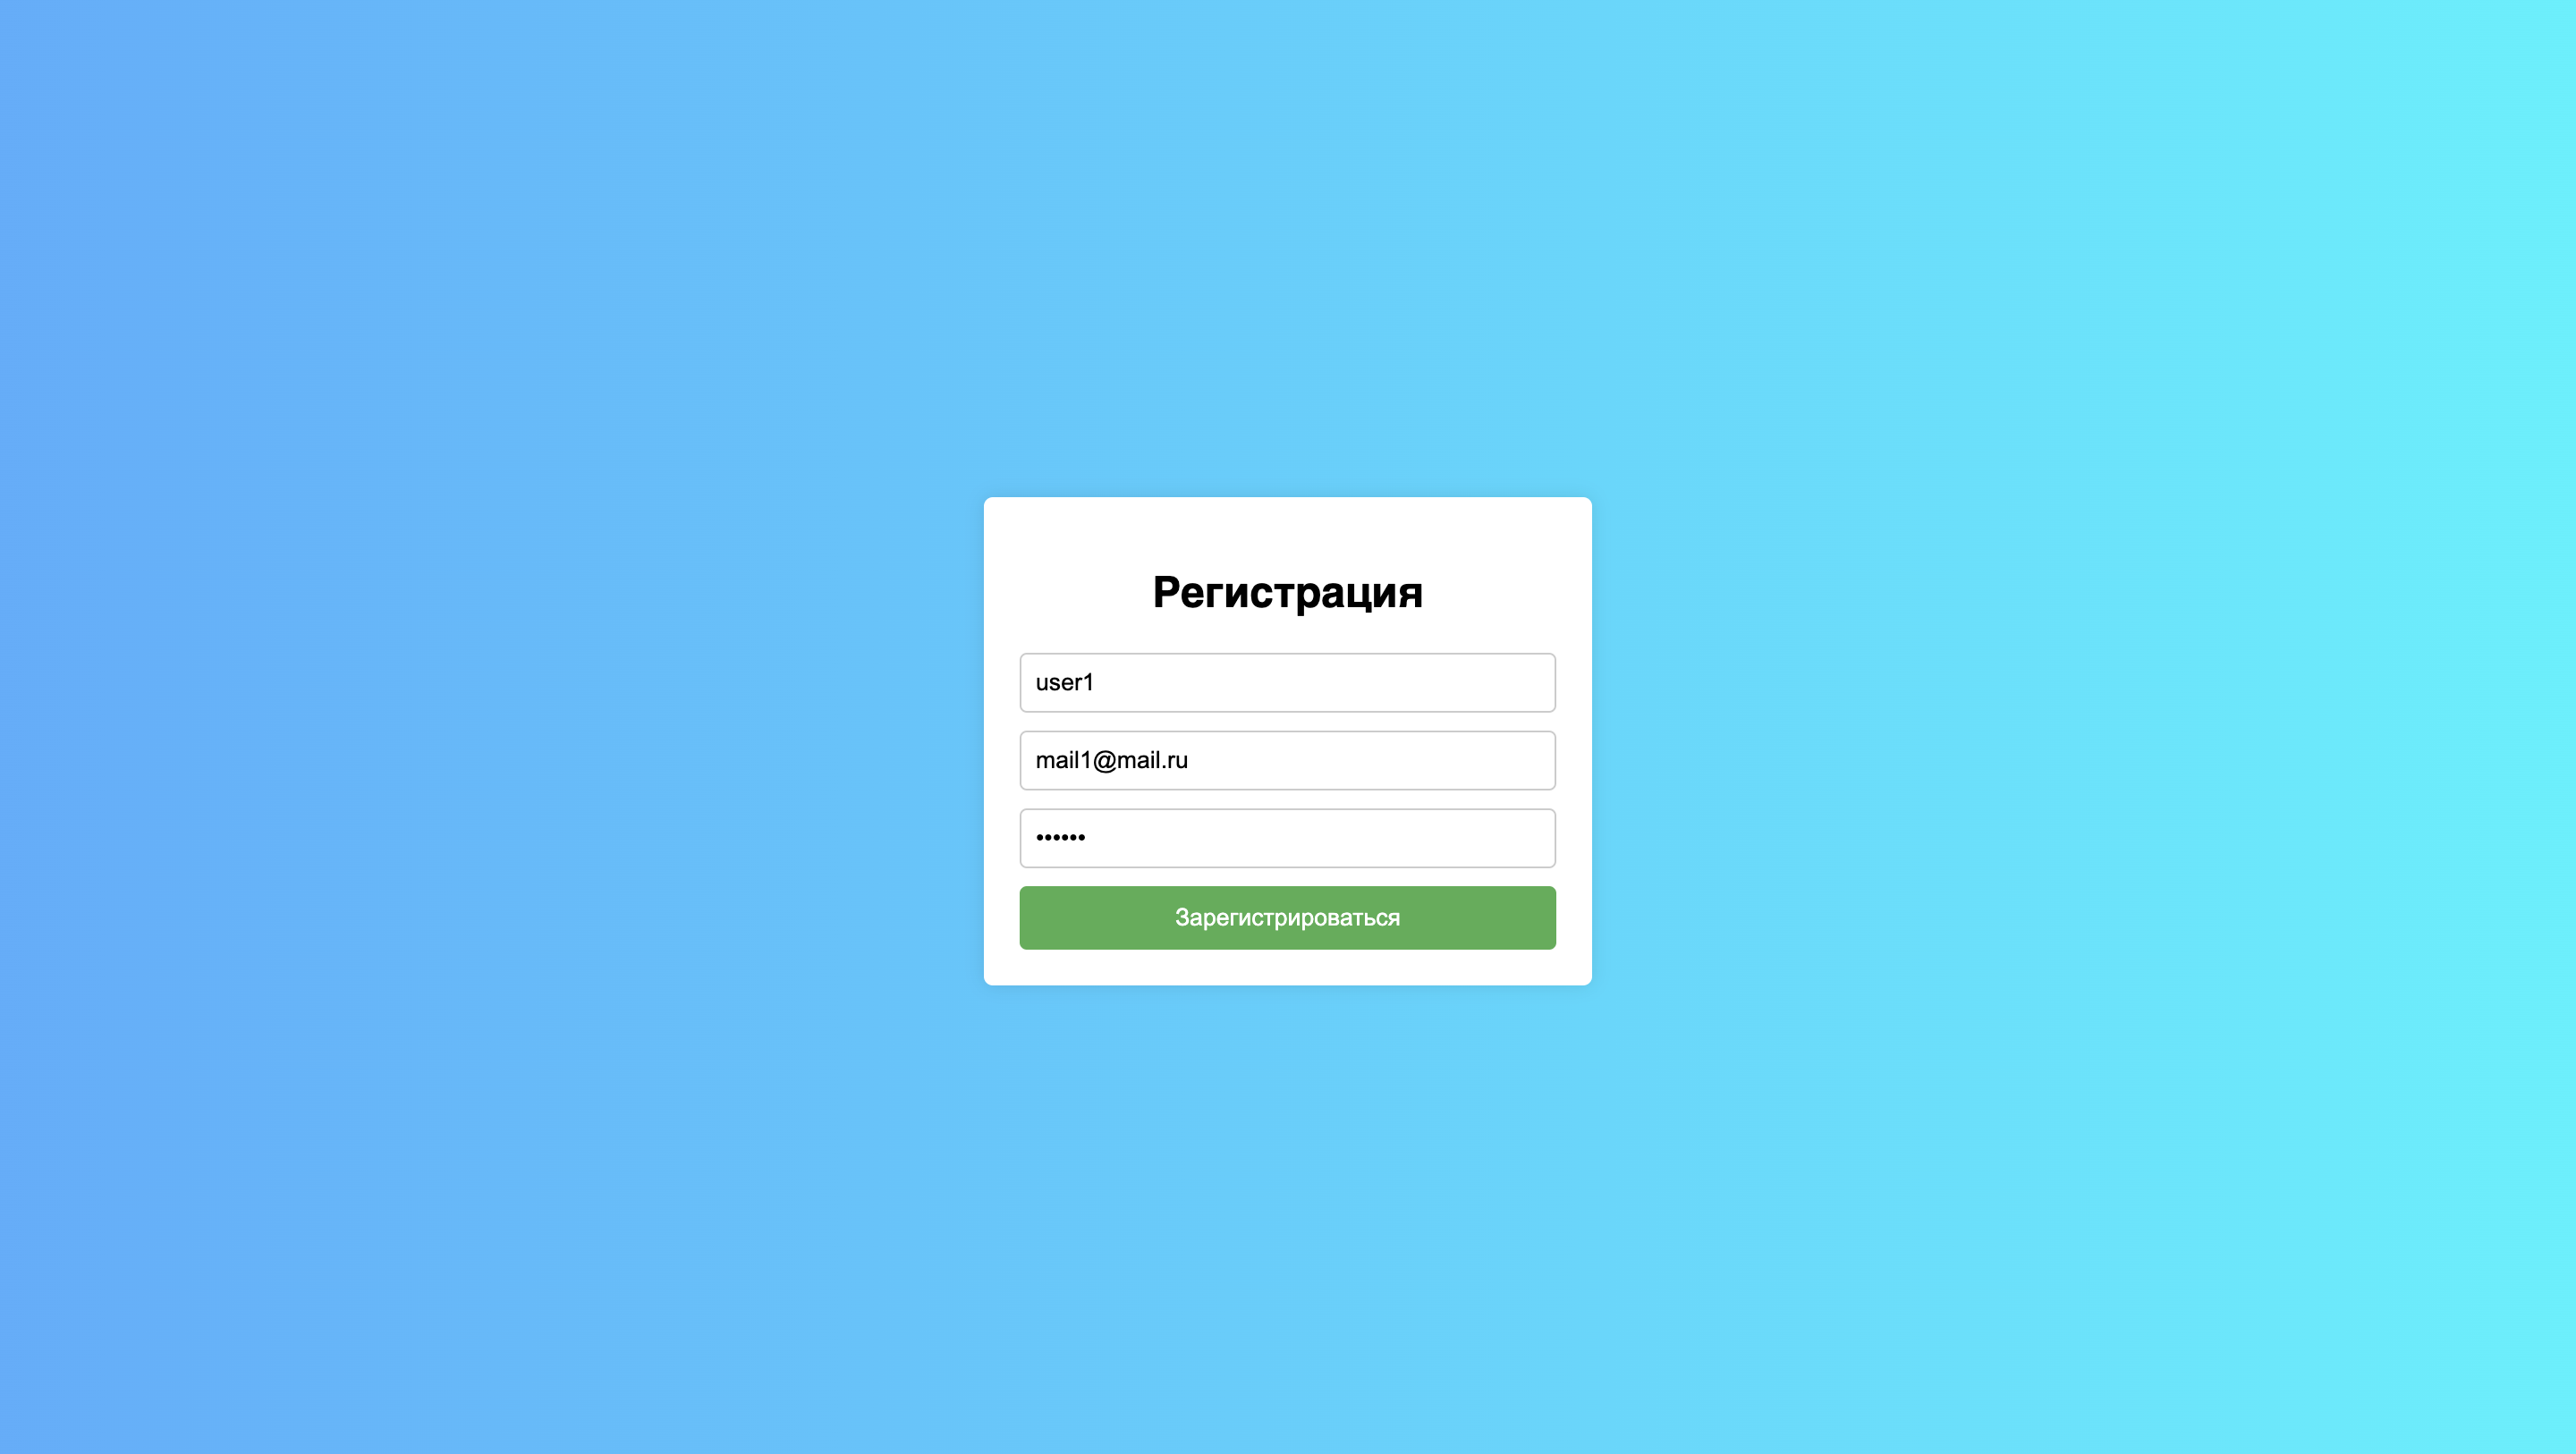
\includegraphics[width=1\linewidth]{img/reg.png}
    \caption{\label{img:reg} Страница для регистрации пользователя}
\end{figure}
\noindent

На рисуне \ref{img:passw} показана страница с восстановлением пароля. Пользователю необходимо ввести почту, которую он использовал при 
регистрации. 

\begin{figure}[H]
    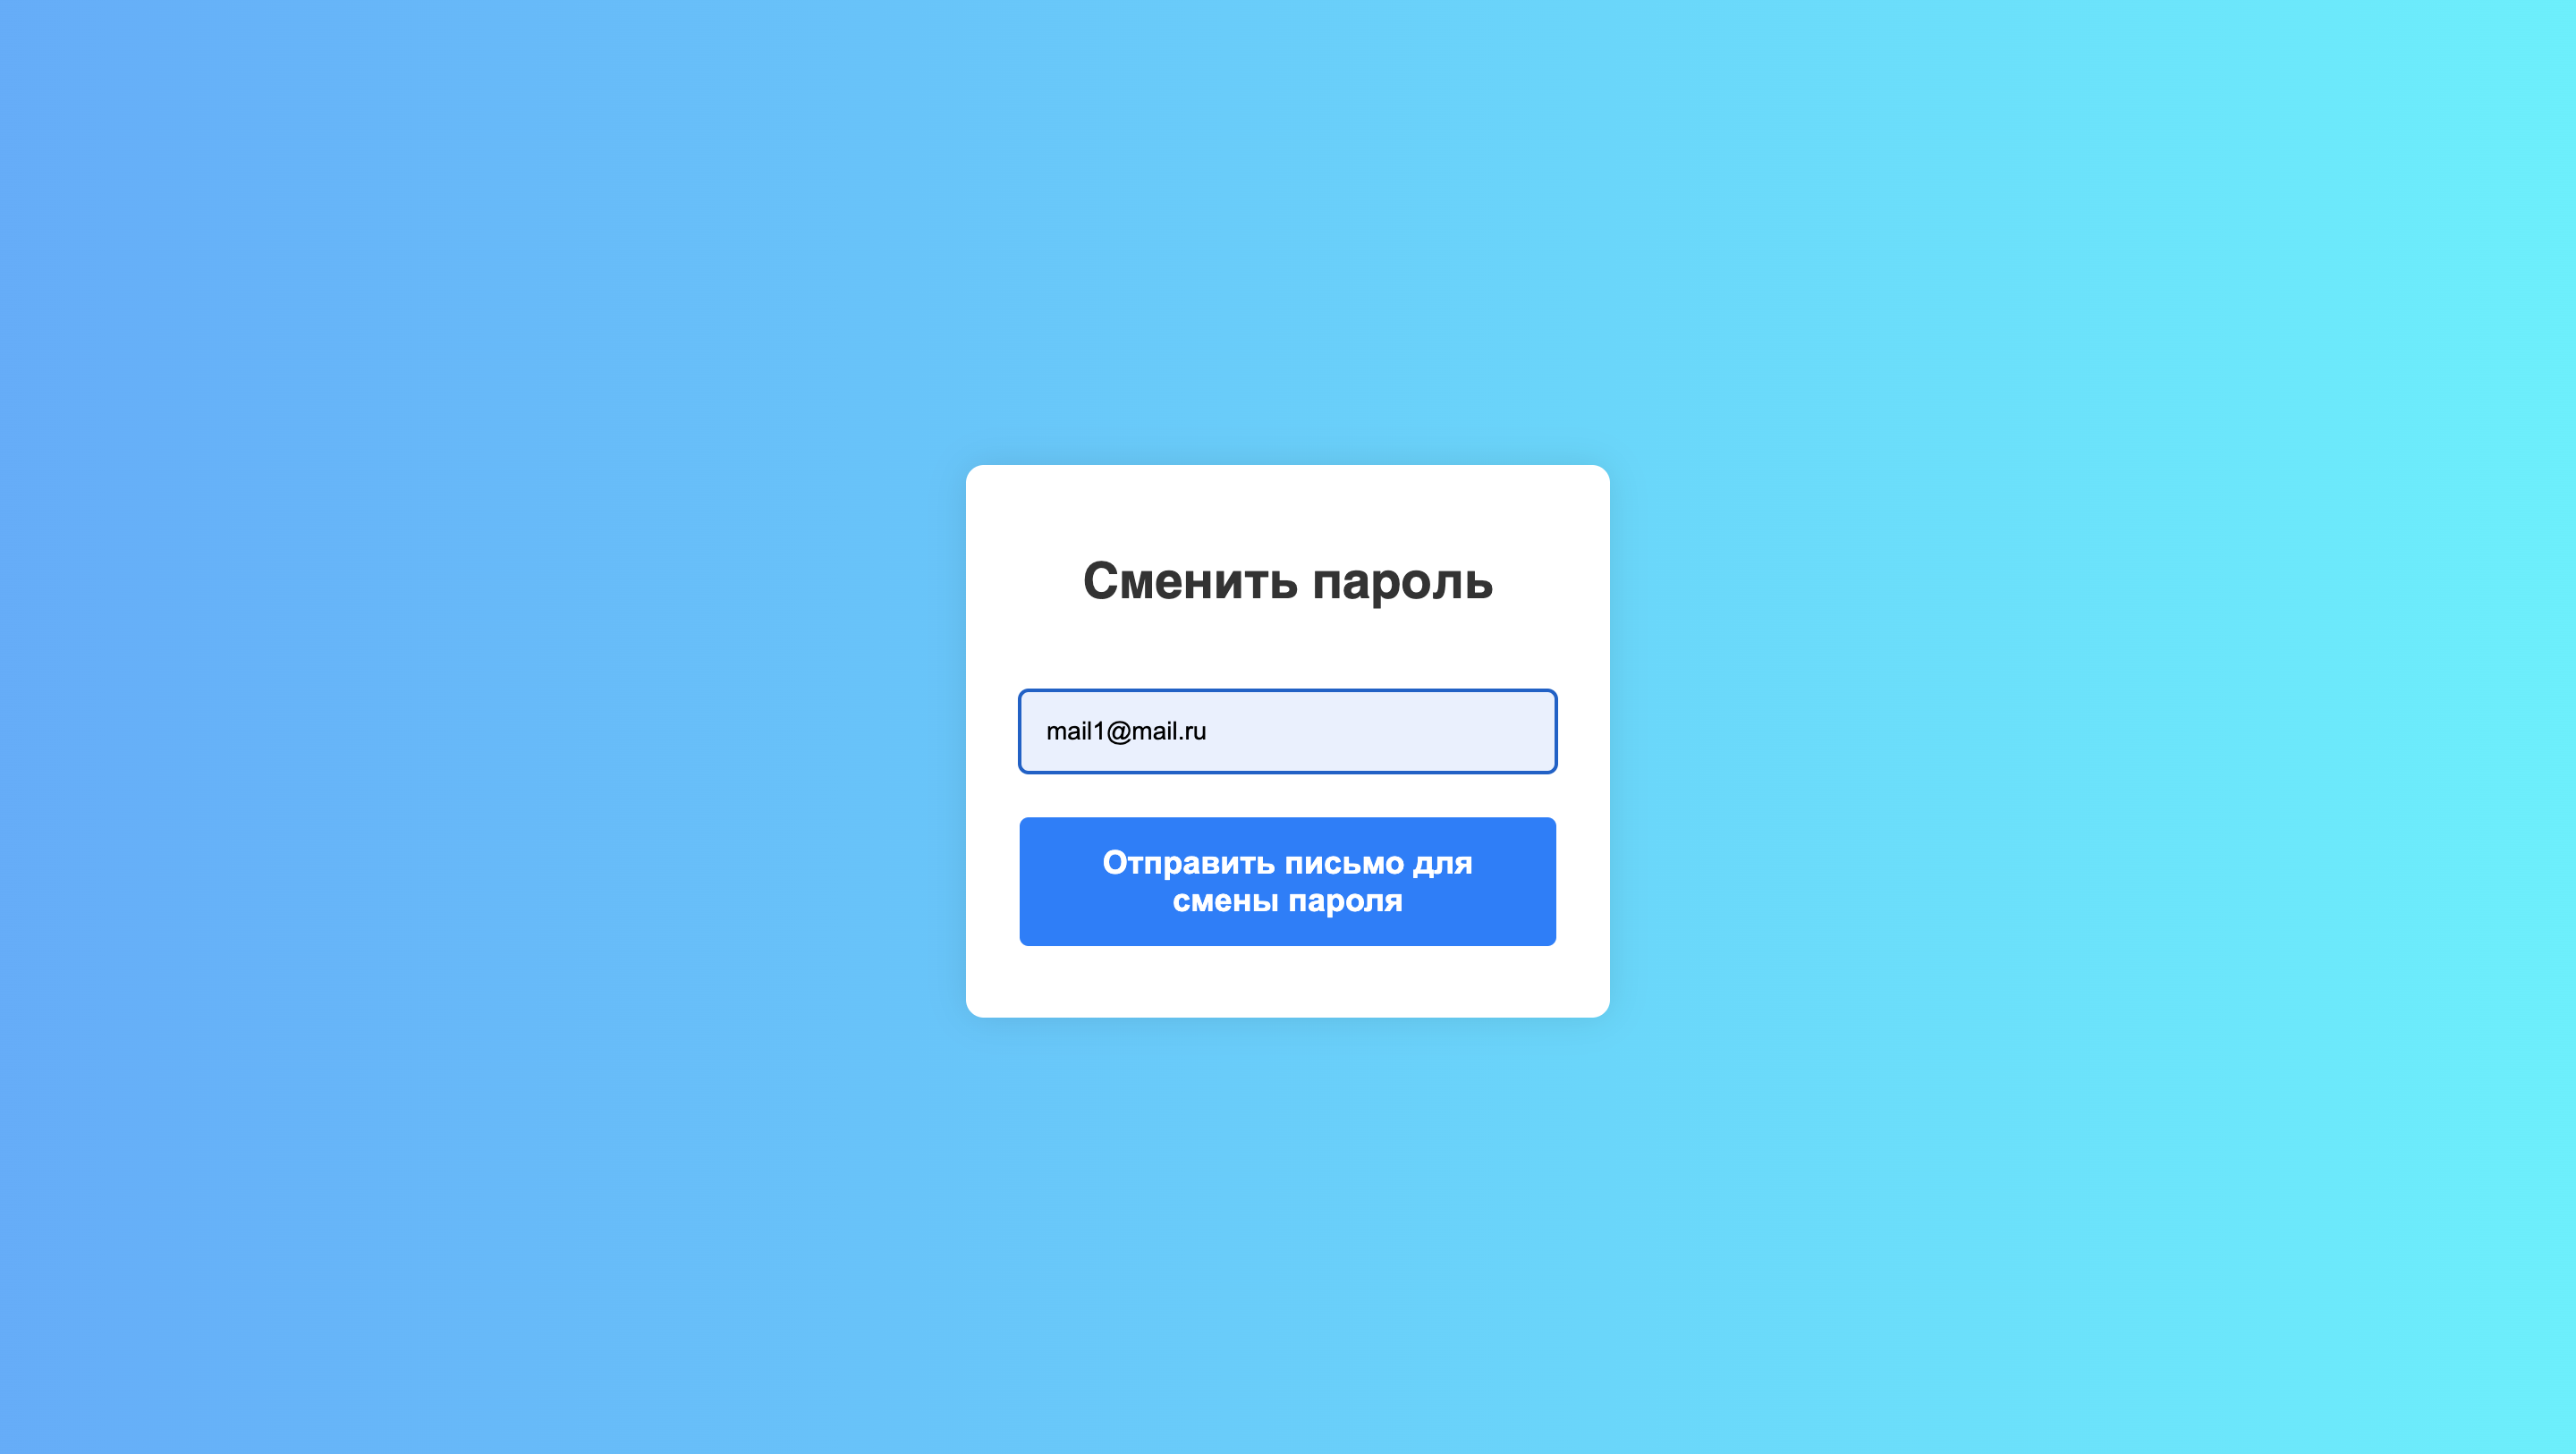
\includegraphics[width=1\linewidth]{img/passw.png}
    \caption{\label{img:passw} Страница с вводом почты для смены пароля}
\end{figure}
\noindent

На указанную почту будет выслан код, который необходимо ввести на странице \ref{img:code}.

\begin{figure}[H]
    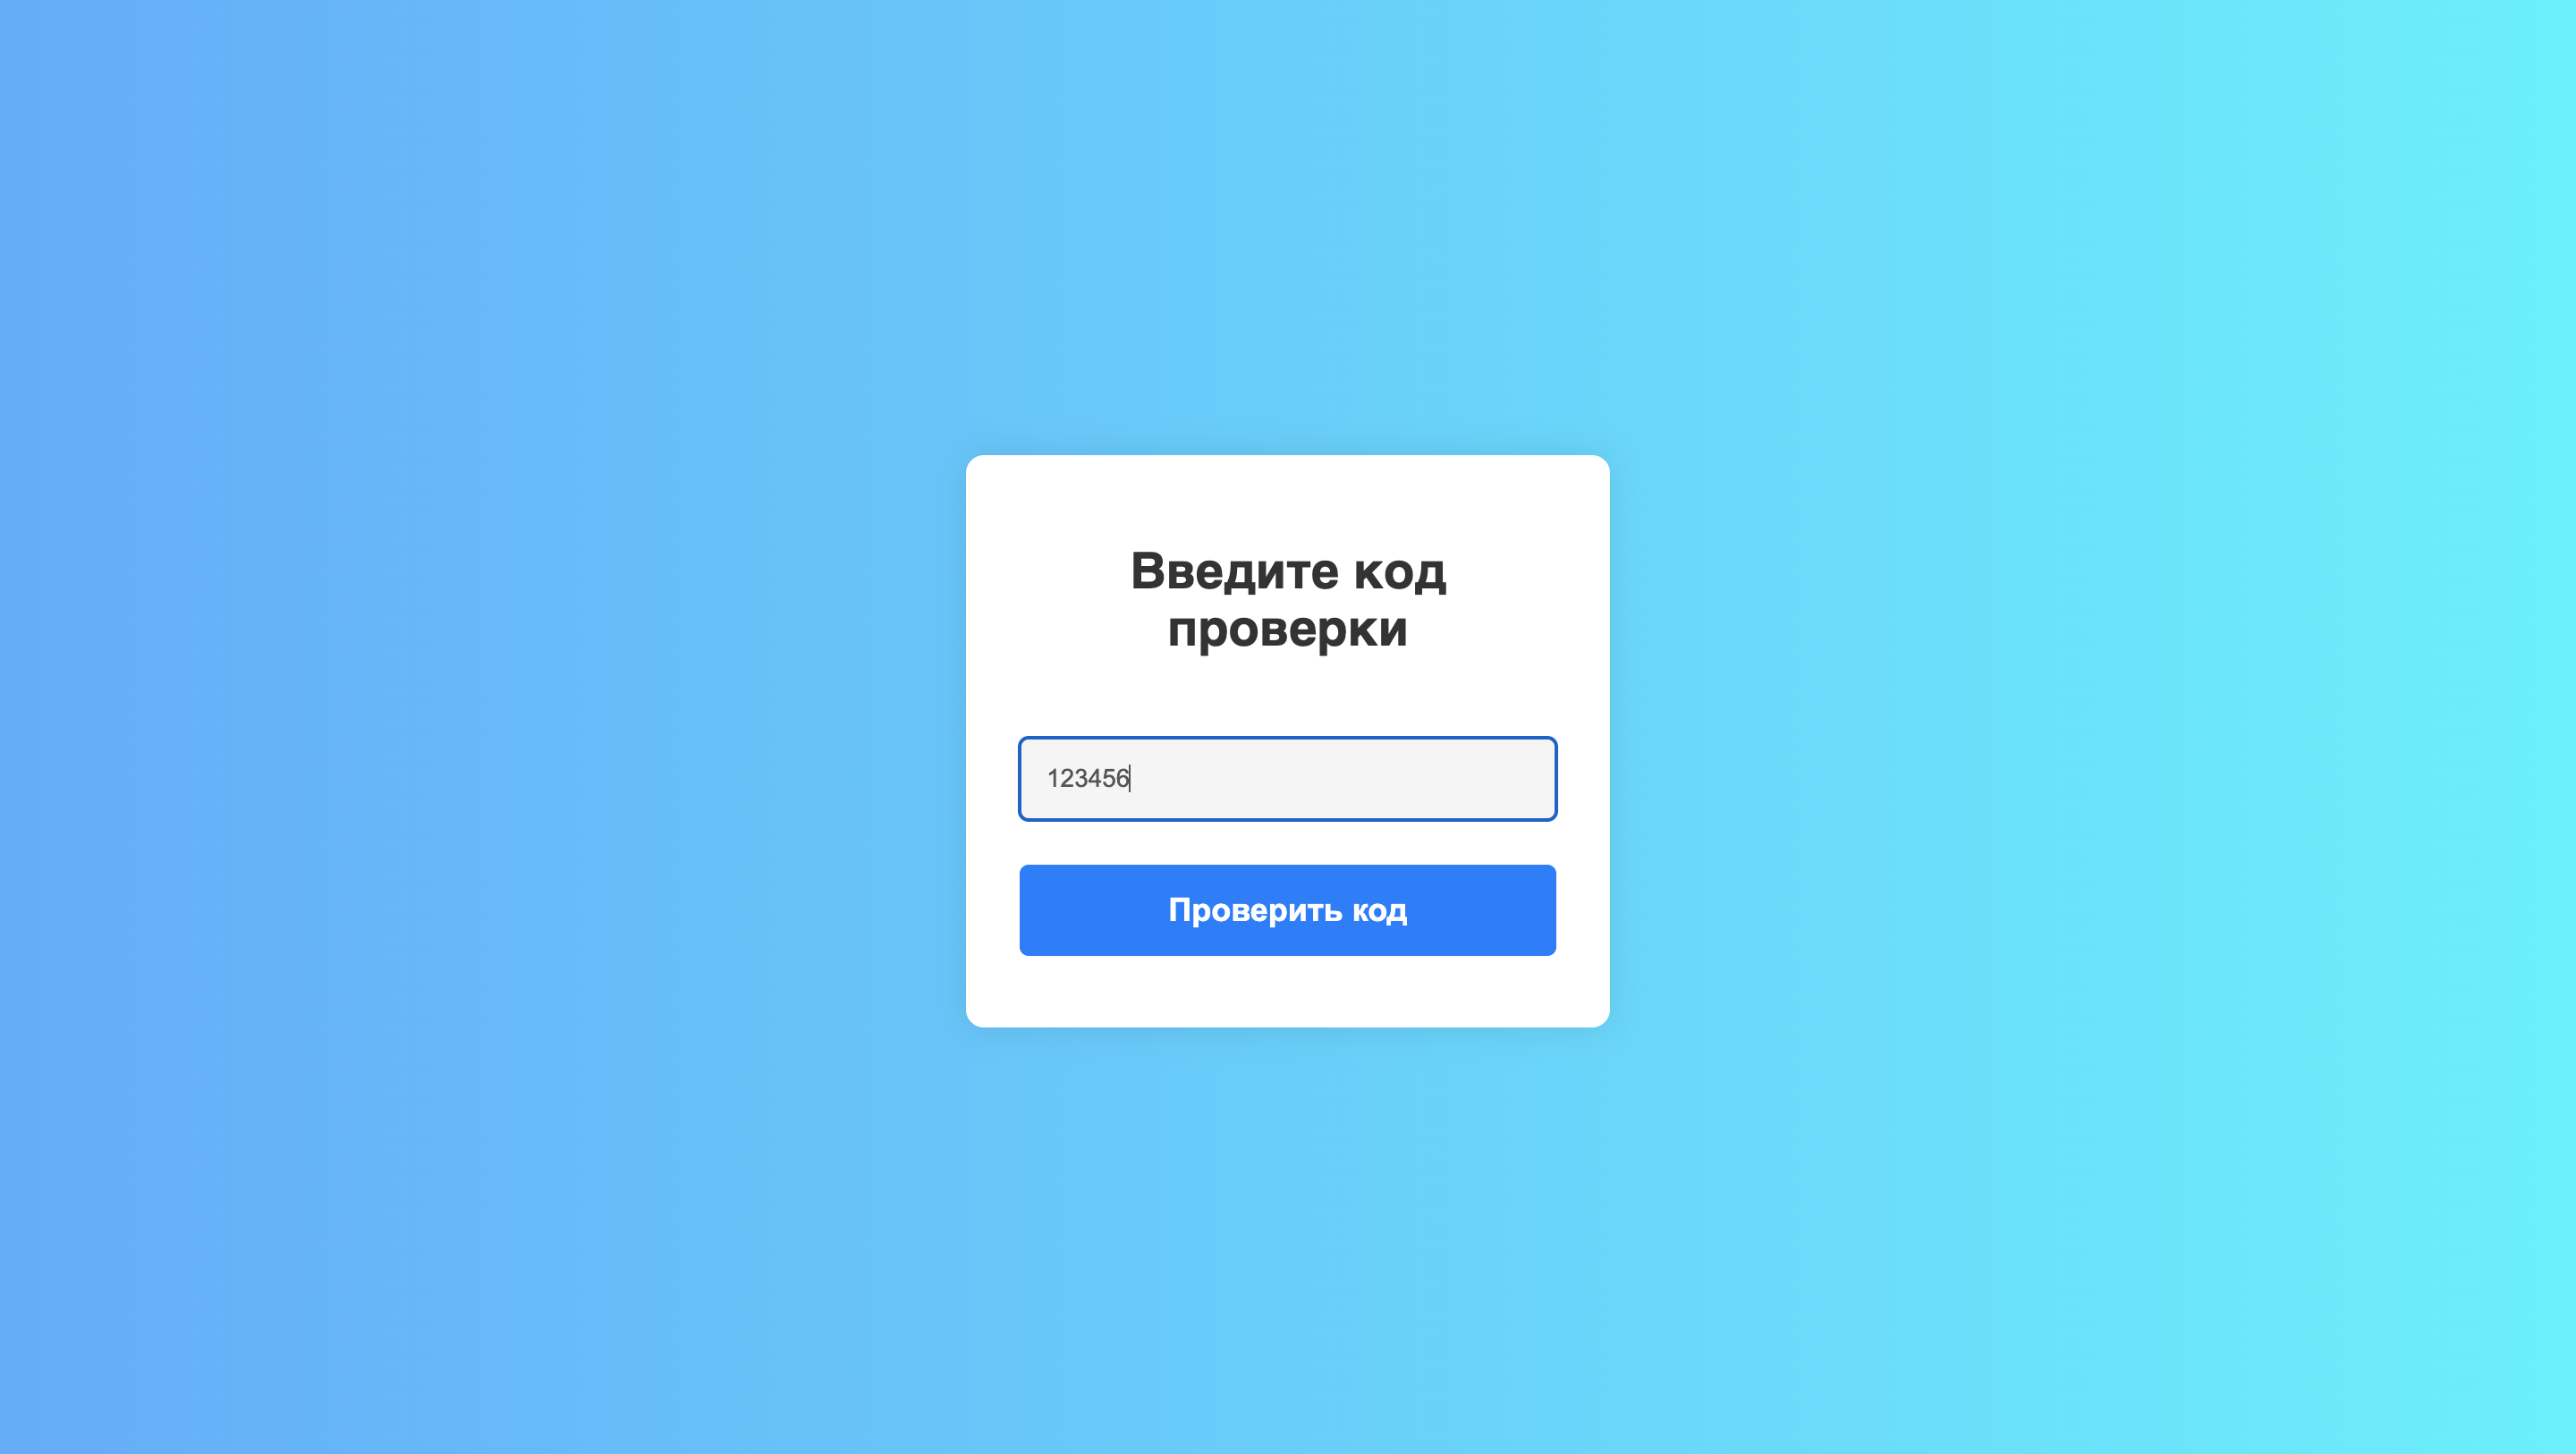
\includegraphics[width=1\linewidth]{img/code.png}
    \caption{\label{img:code} Страница с вводом кода проверки}
\end{figure}
\noindent

Далее пользователю будет предложено сменить пароль \ref{img:smena}.

\begin{figure}[H]
    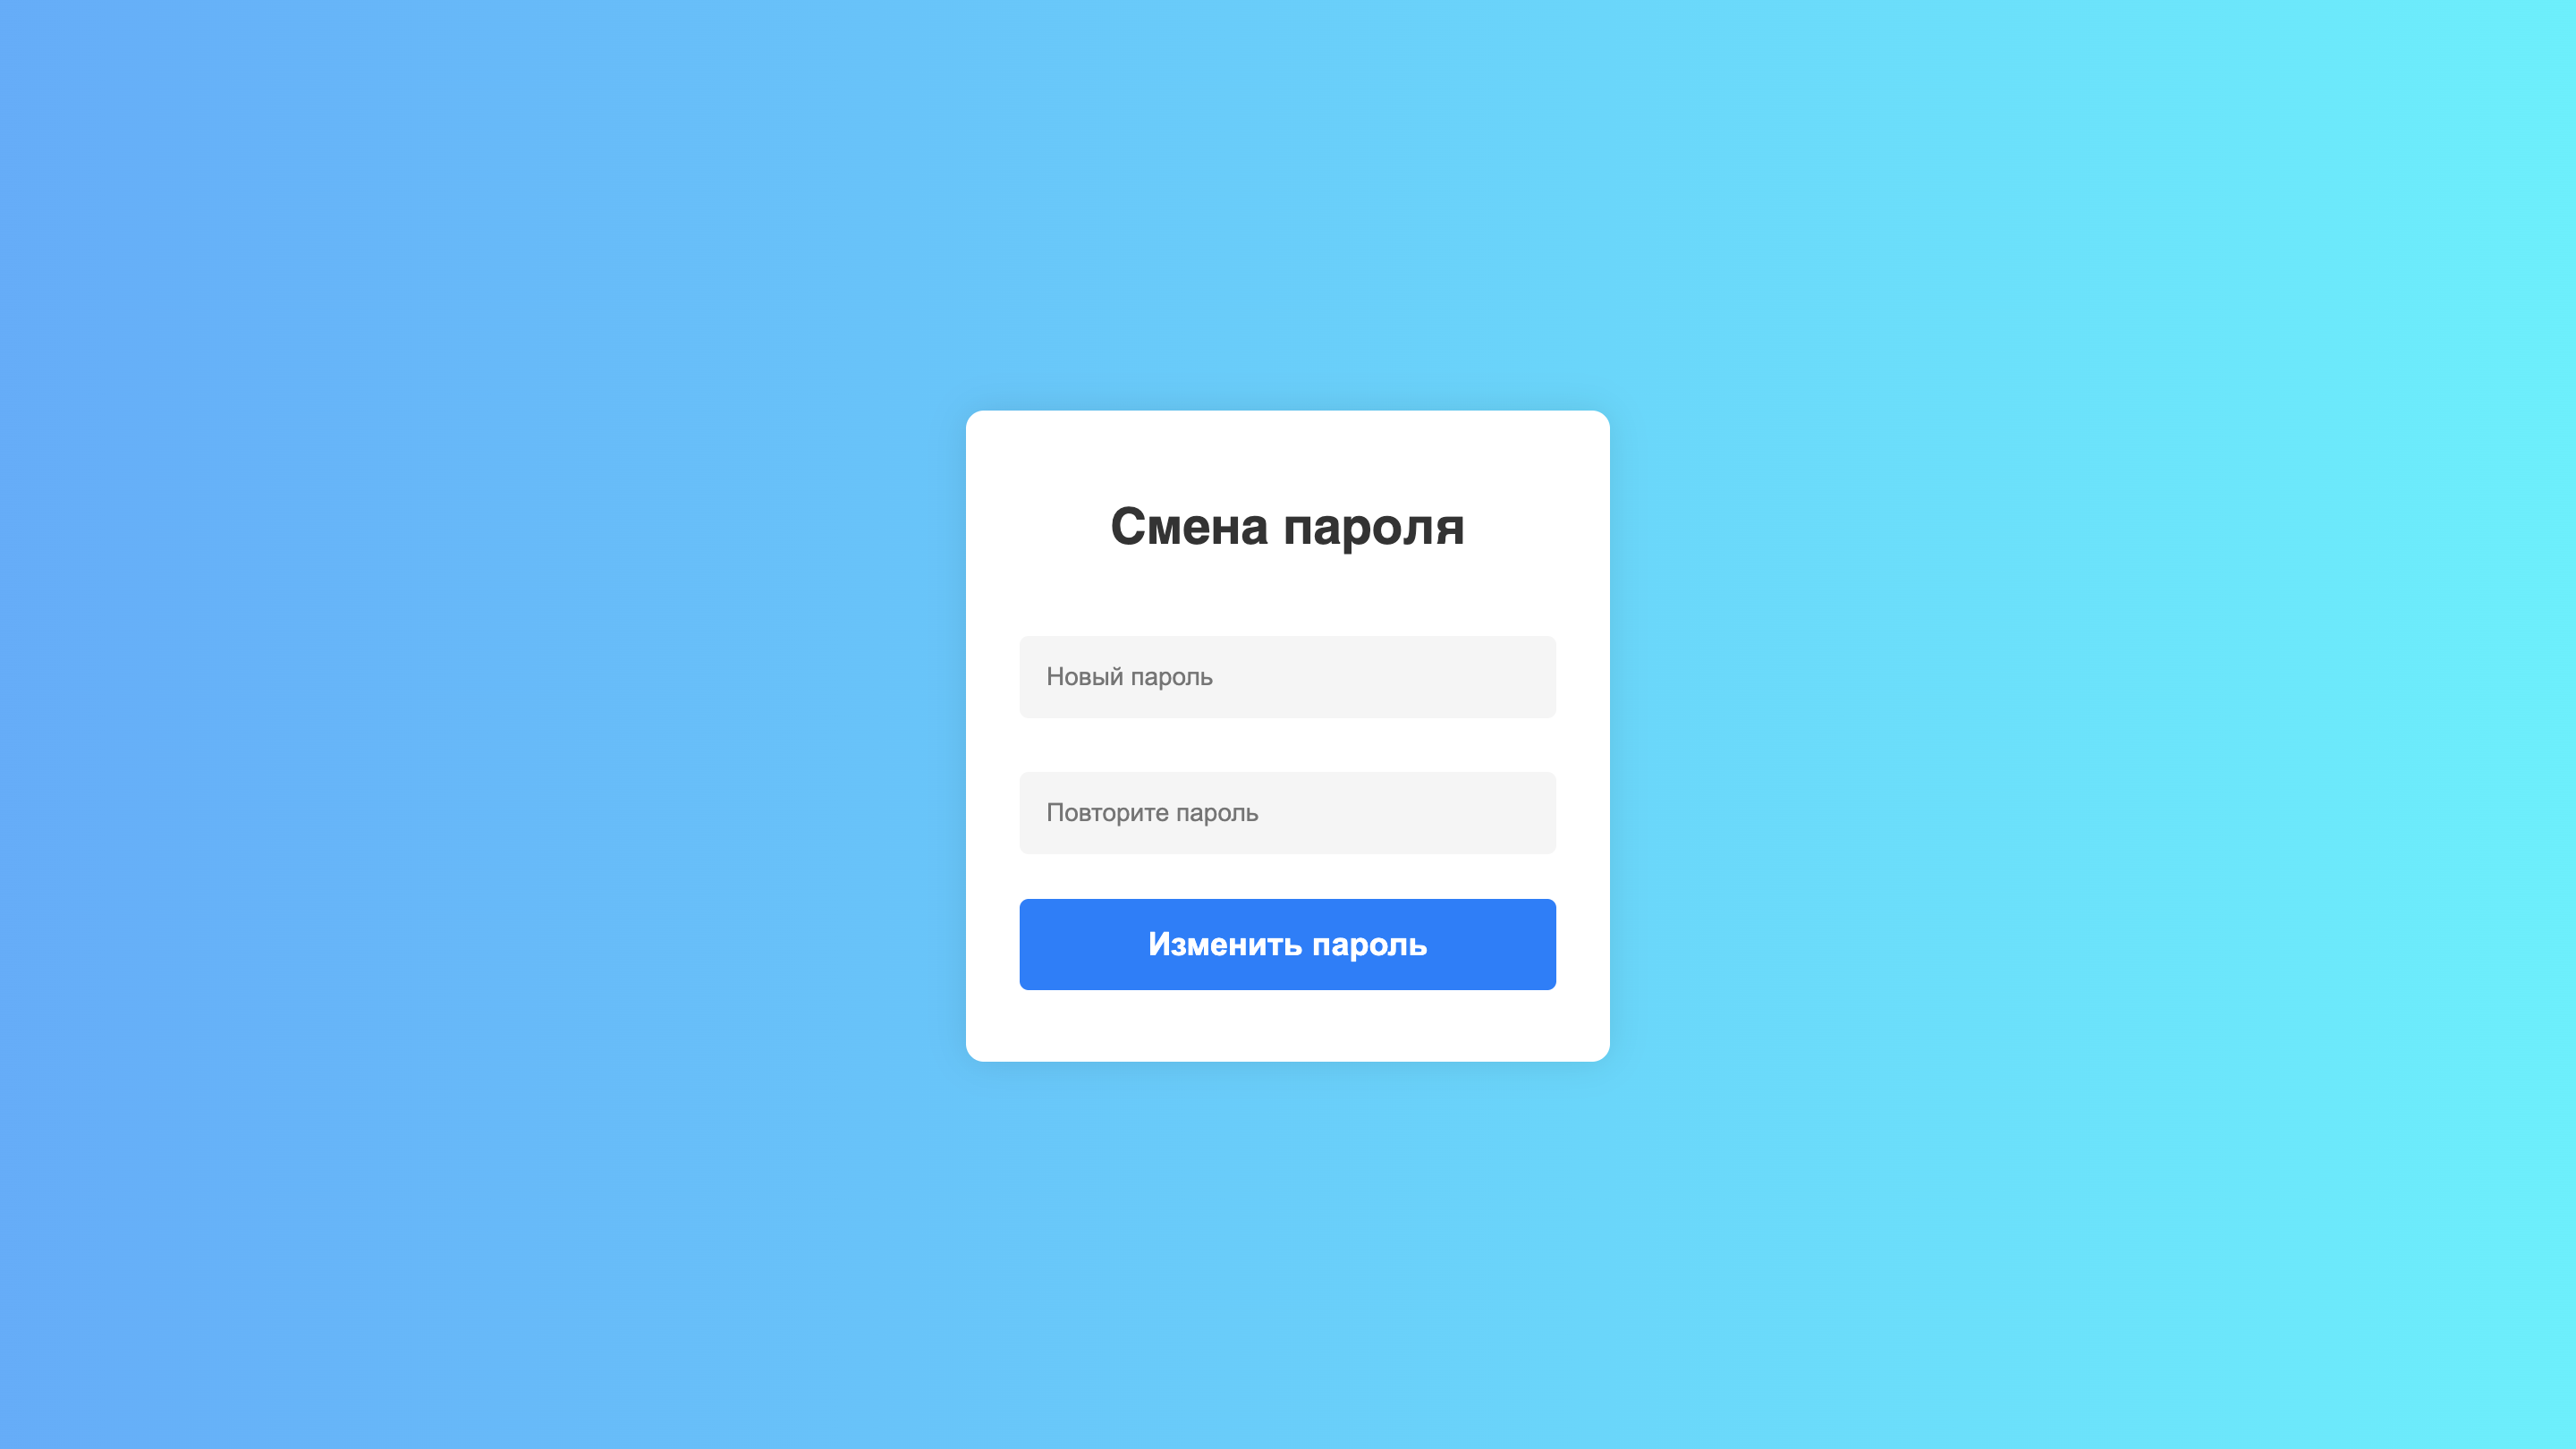
\includegraphics[width=1\linewidth]{img/smena.png}
    \caption{\label{img:smena} Страница со сменой пароля}
\end{figure}
\noindent

После авторизации пользователь будет перемещен в меню, которое содержит кнопки для перехода на 
страницы дома, устройств и прав доступа \ref{img:menu}.

\begin{figure}[H]
    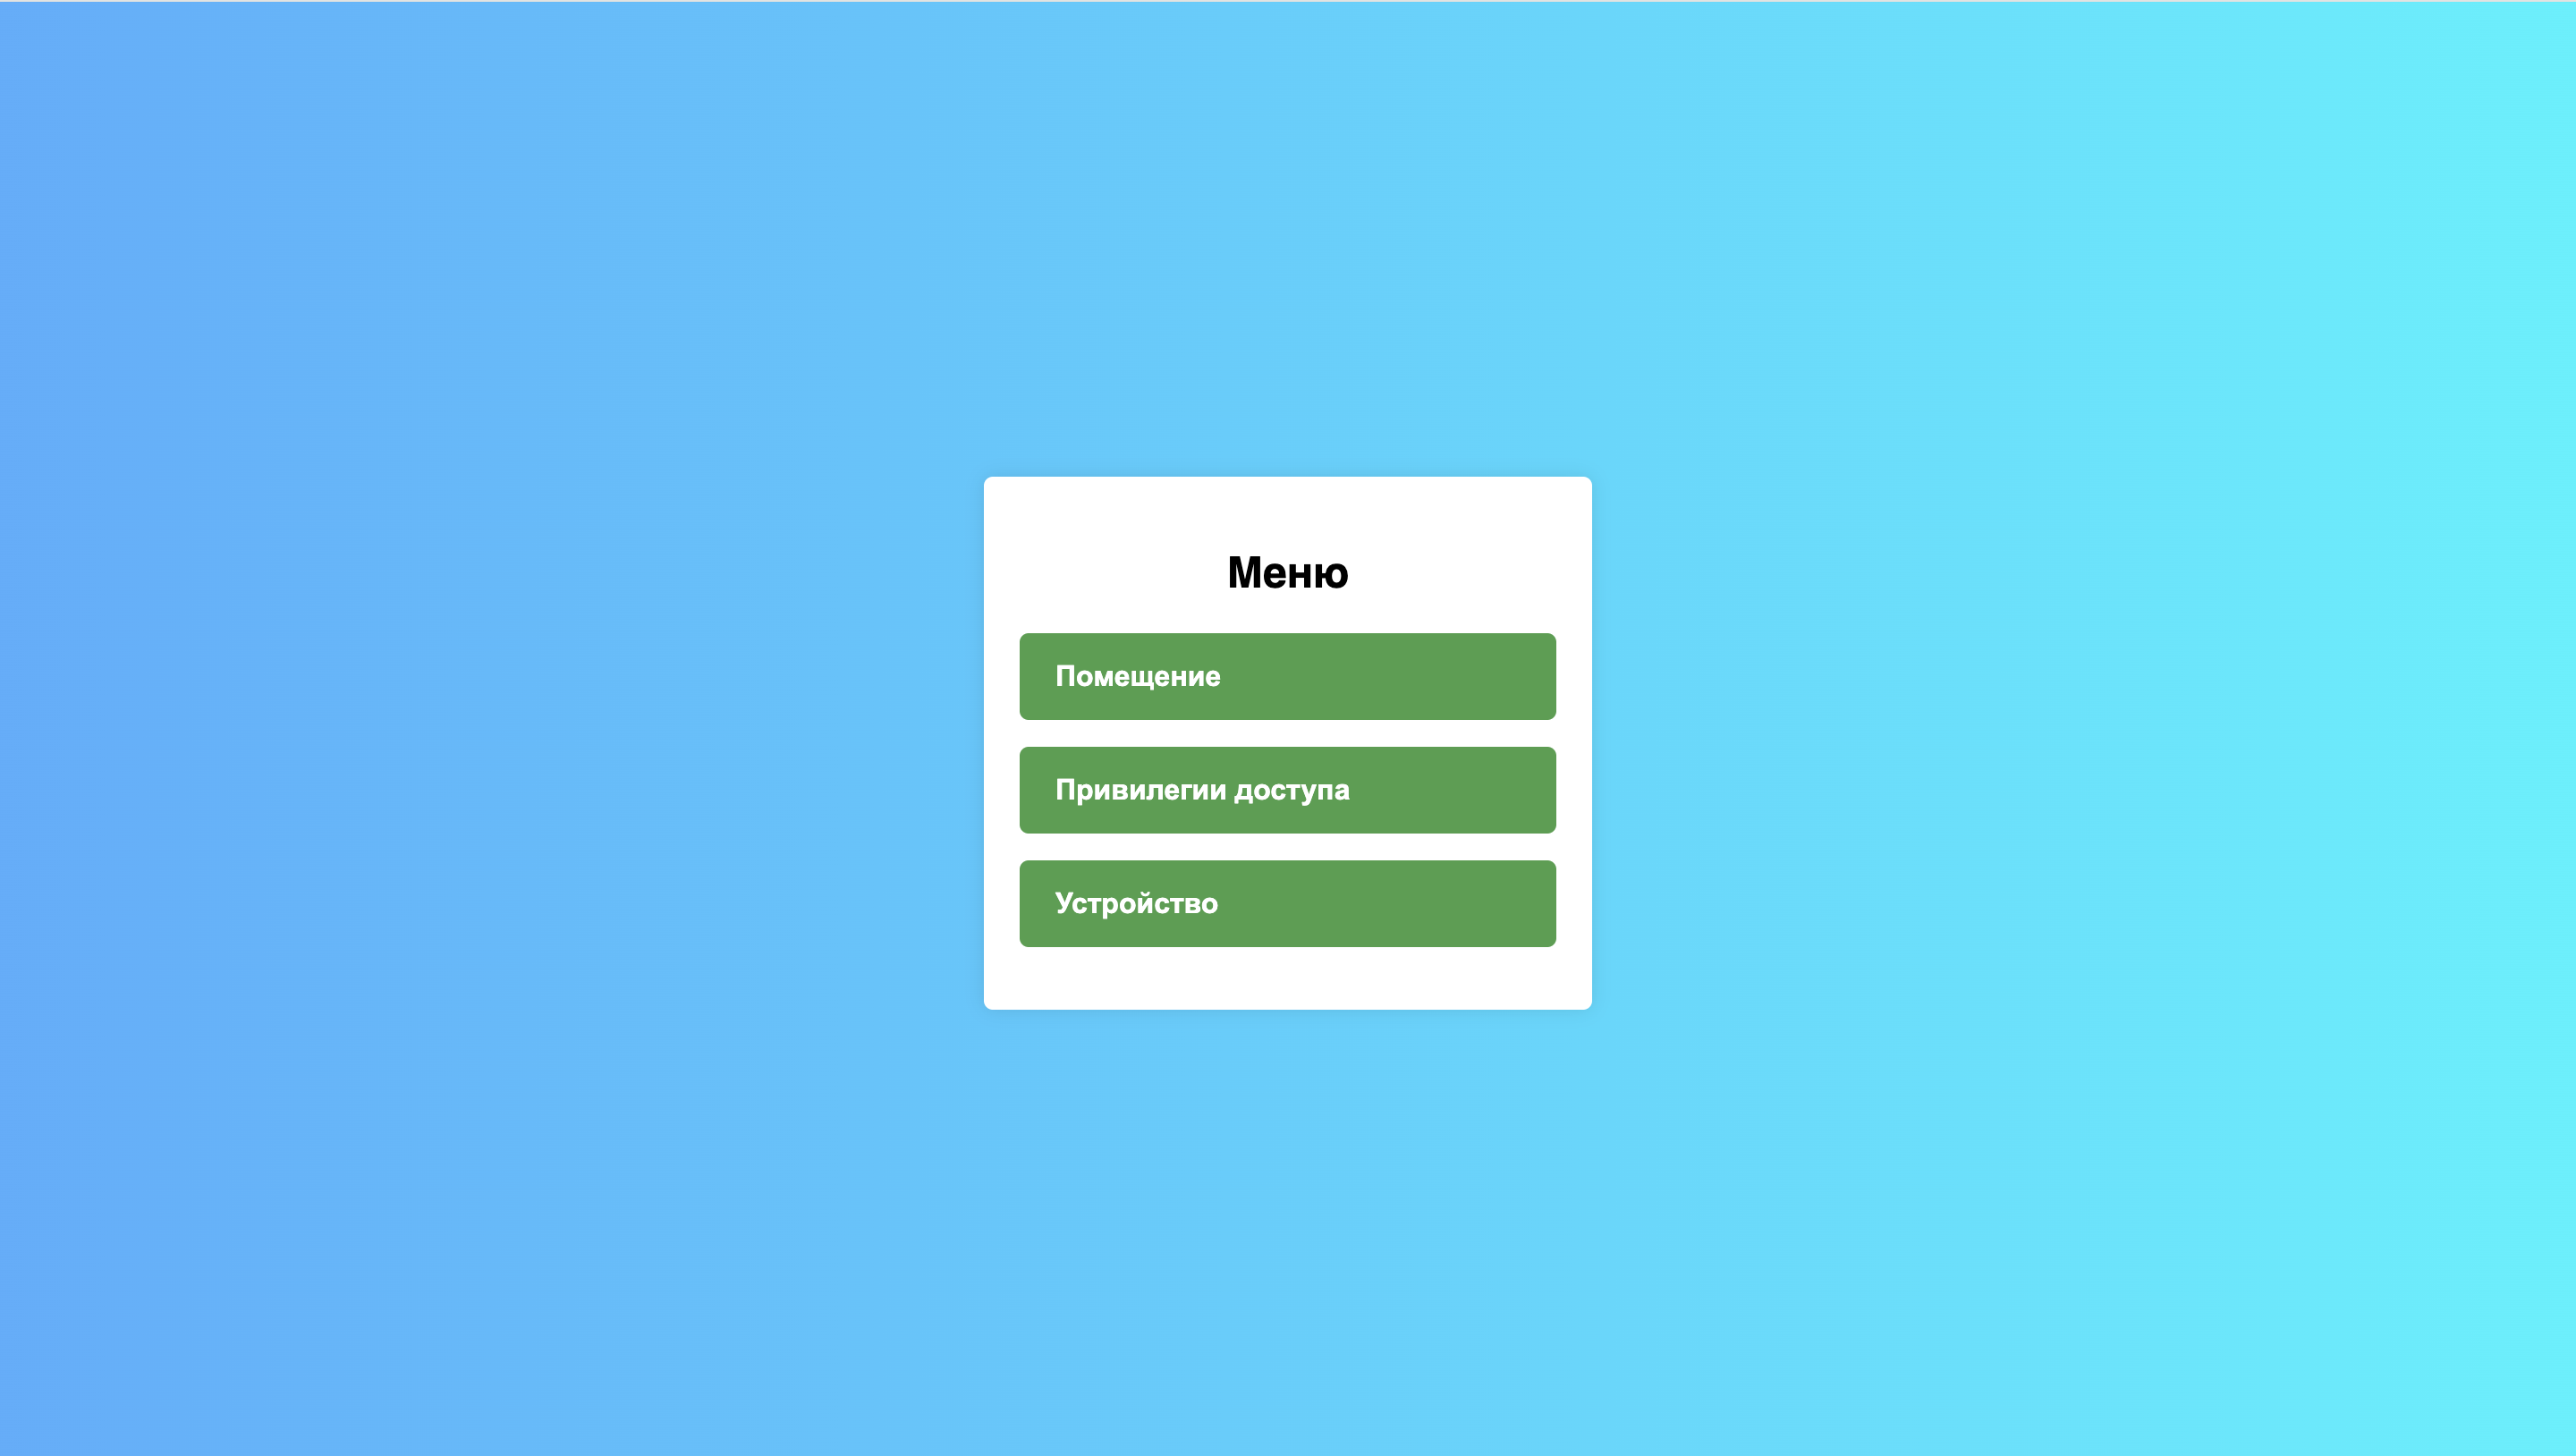
\includegraphics[width=1\linewidth]{img/menu.png}
    \caption{\label{img:menu} Страница со сменой пароля}
\end{figure}
\noindent

При нажатии на кнопу «Помещение» пользователь перейдет на страницу управления домом \ref{img:home}. На данной странице 
предоставляется возможность создать или удалить дом, обновить его имя, а также просмотреть список домов, которыми владеет 
пользователь. 

\begin{figure}[H]
    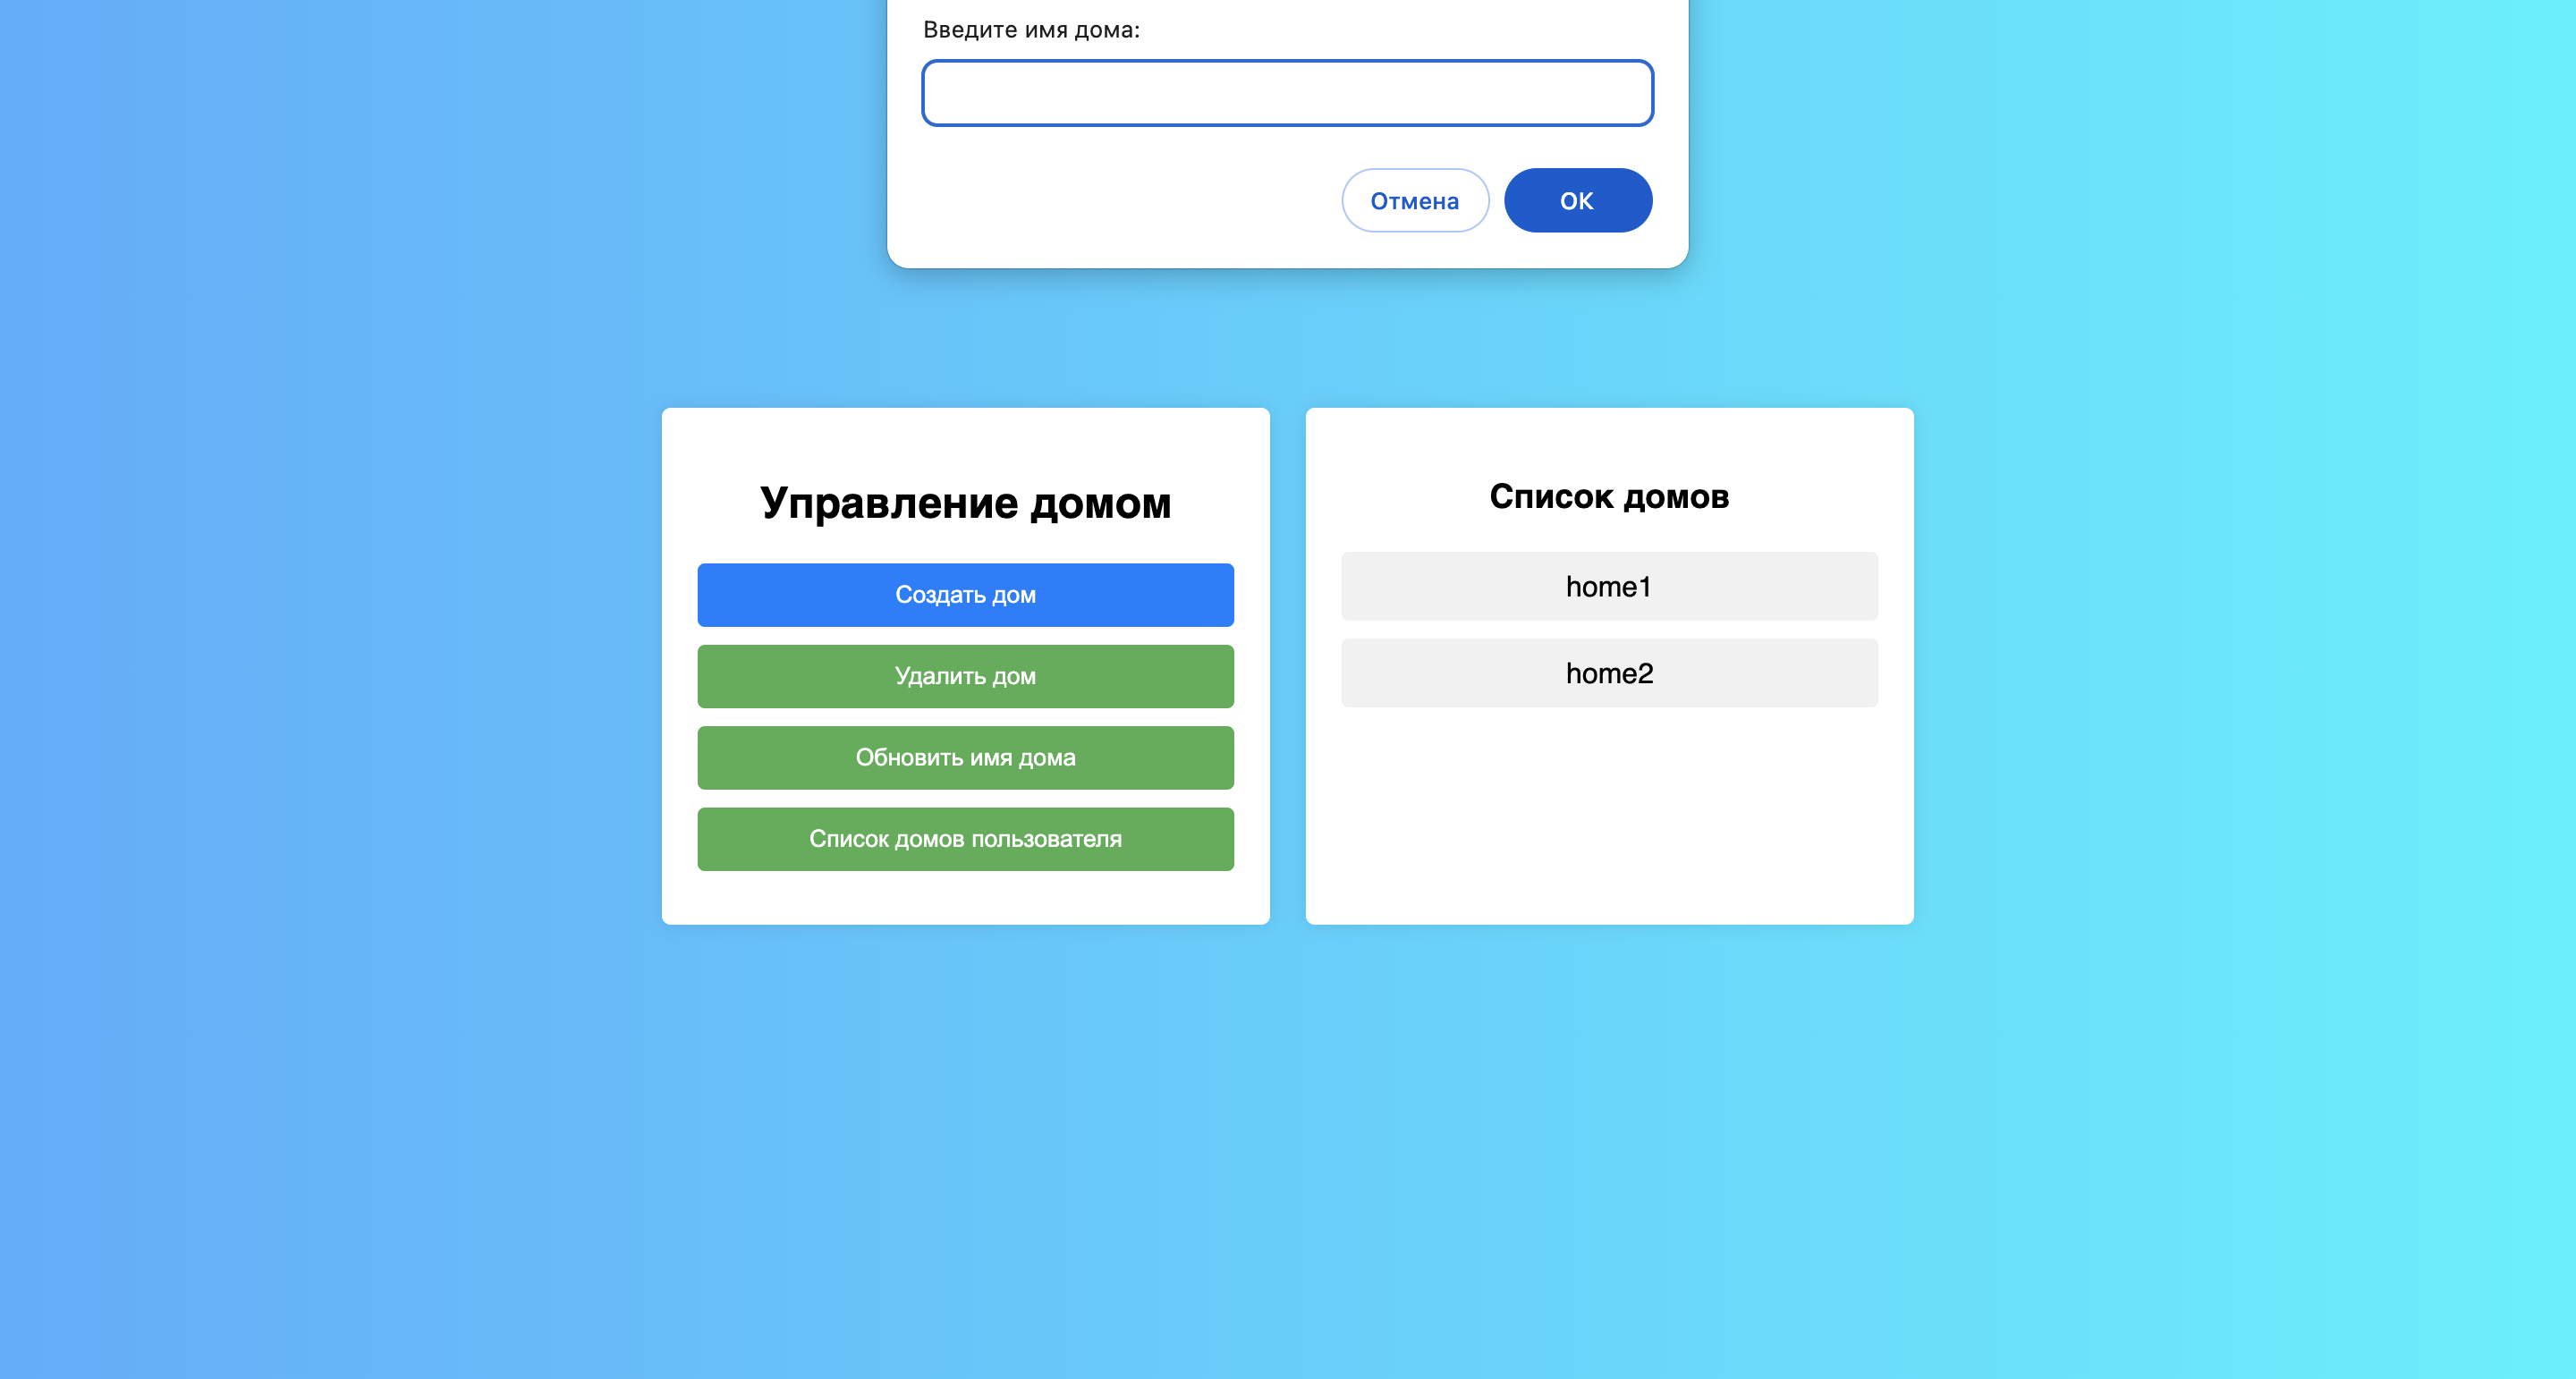
\includegraphics[width=1\linewidth]{img/home.png}
    \caption{\label{img:home} Страница для управления домом}
\end{figure}
\noindent

При нажатии на кнопку «Привилегии доступа» пользователь переходит на страницу, которая предоставляет возможность
управлять многопользовательским режимом \ref{img:access}. На данной странцие владелец дома может
добавить новых участников или удалить их. Также ему предоставляется возможность
просмотреть список участников дома и обновить уровень доступа участника.

\begin{figure}[H]
    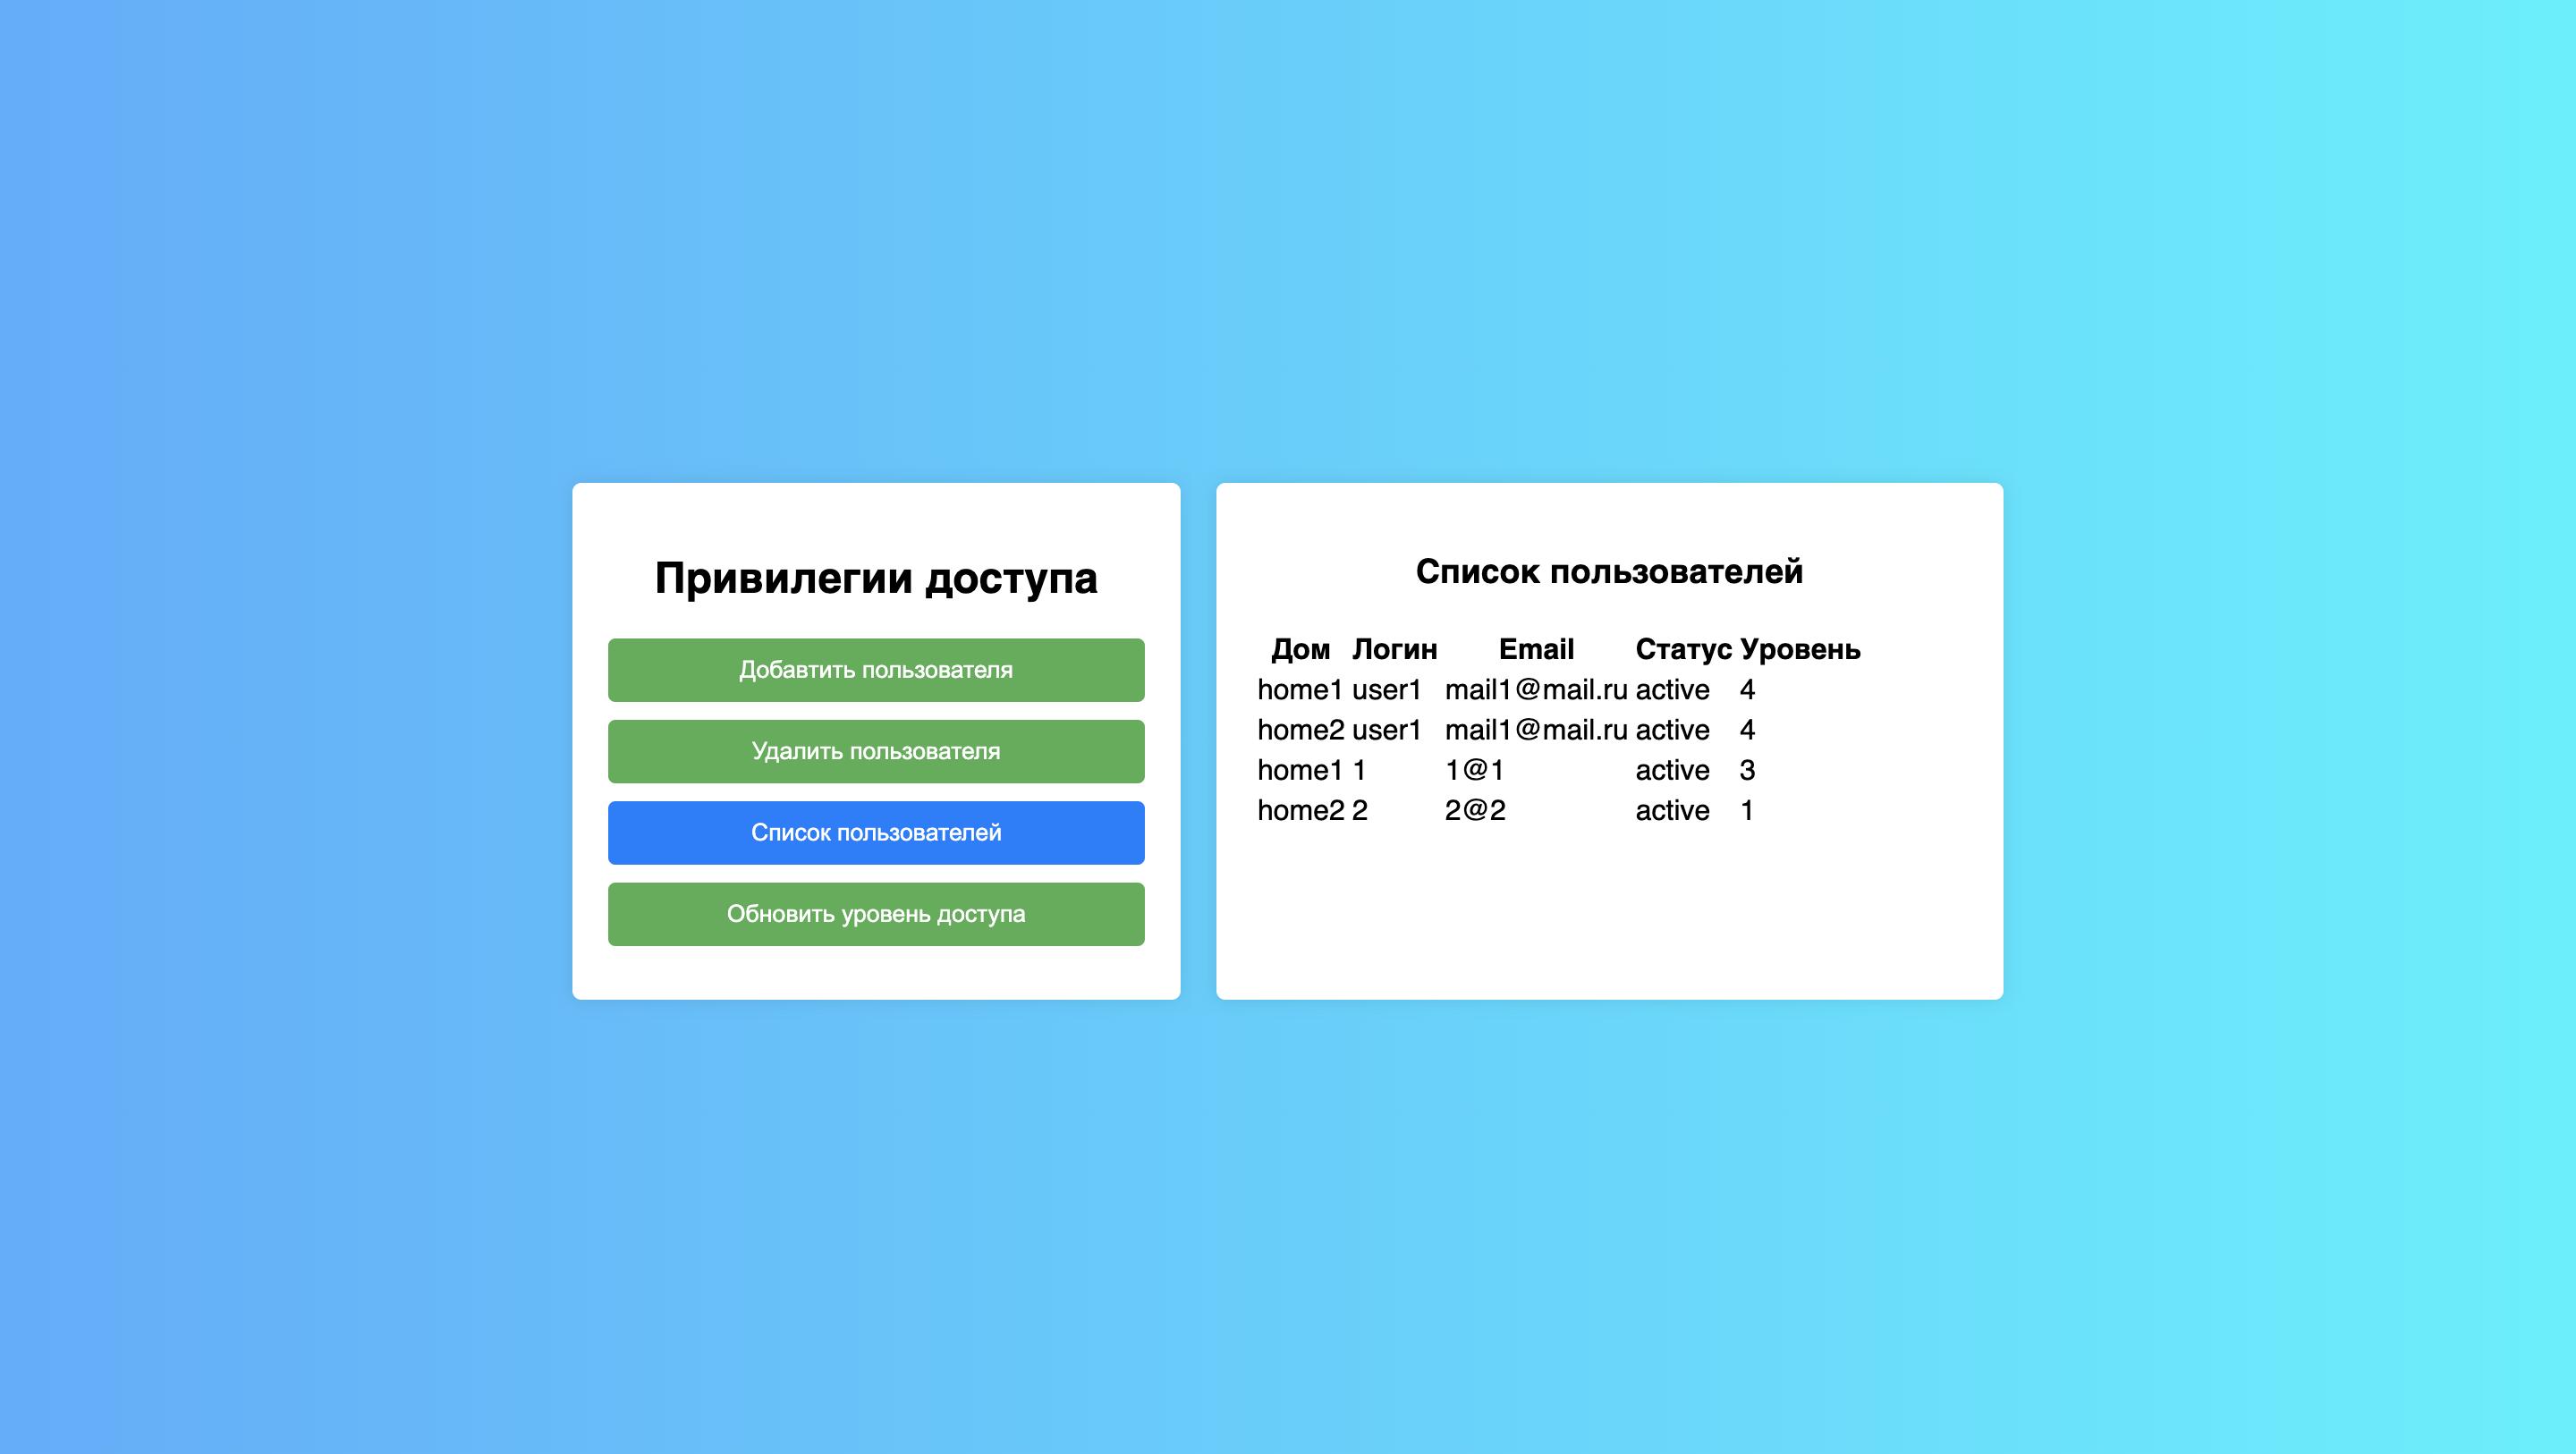
\includegraphics[width=1\linewidth]{img/access.png}
    \caption{\label{img:access} Страница многопользовательского режима}
\end{figure}
\noindent

При нажатии на кнопу «Устройство» пользователь переходит на страницу управления устройствами \ref{img:dev}. На данной странице 
пользователь может добавить новое устройство в свой дом или удалить уже добавленное. Также ему предоставляется возможность
просмотреть список устройств, запустить устройство и просмотреть историю работы устройства.

\begin{figure}[H]
    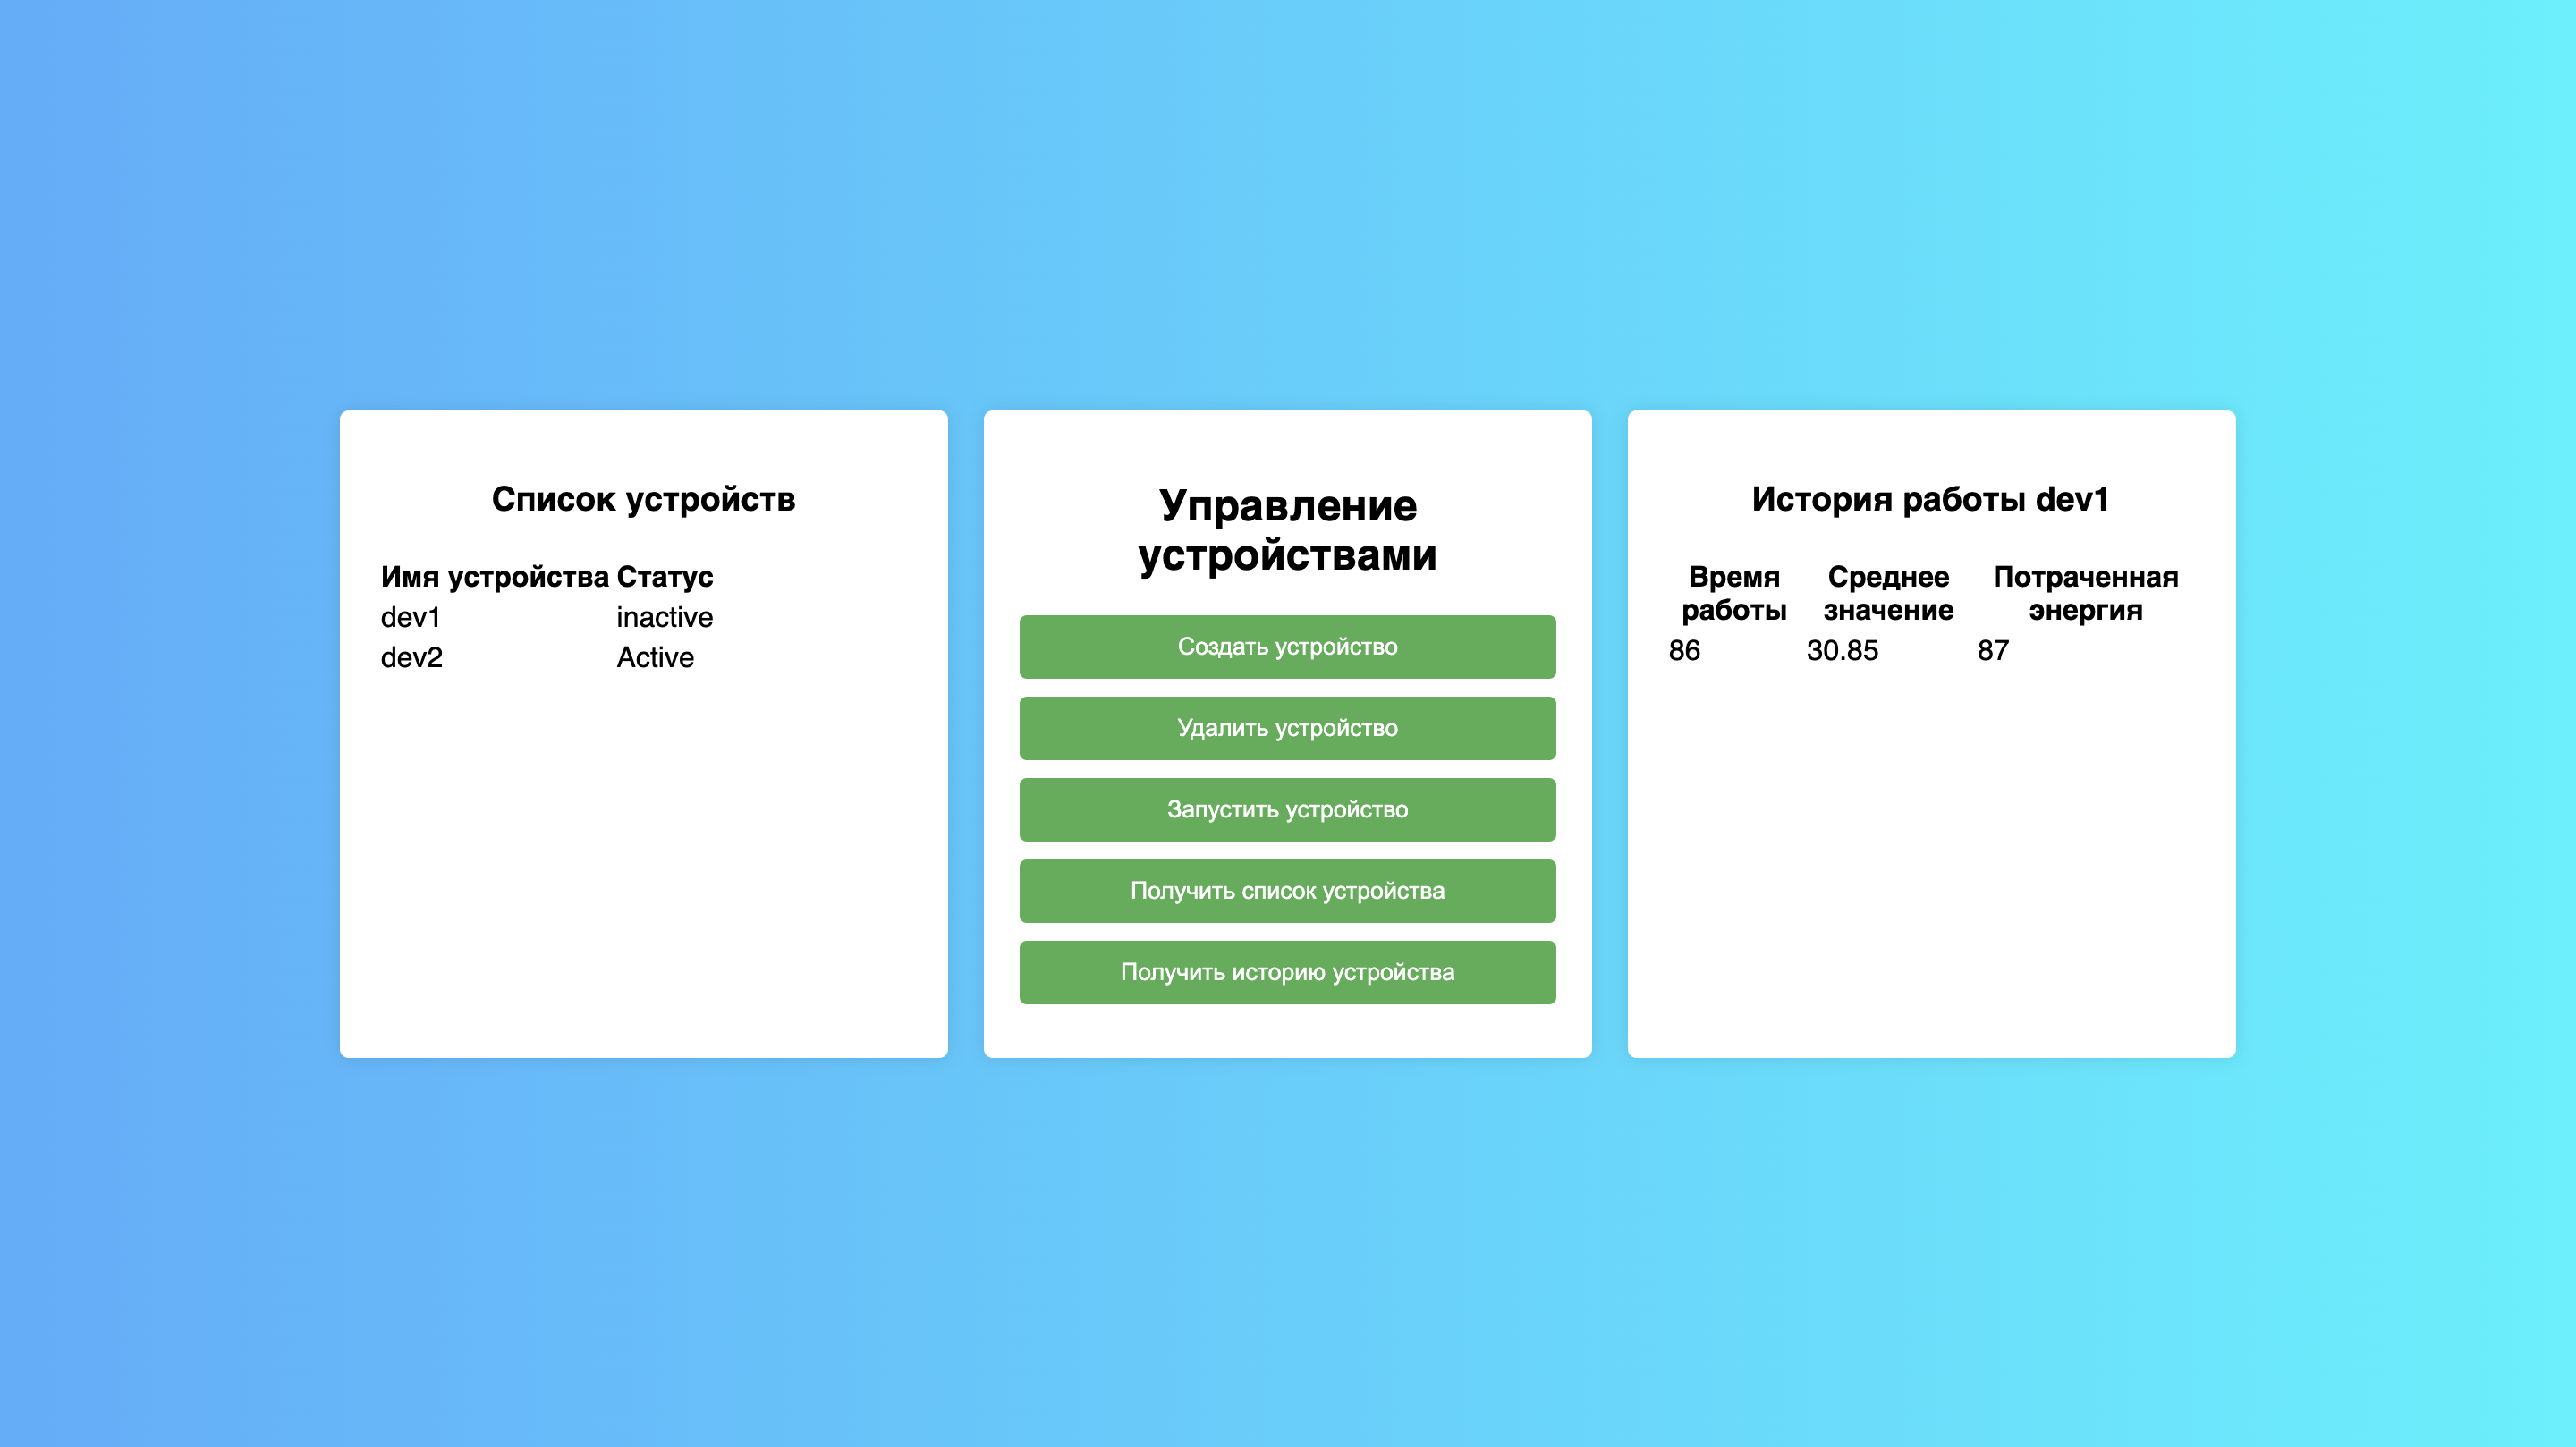
\includegraphics[width=1\linewidth]{img/device.png}
    \caption{\label{img:dev} Страница управления устройством}
\end{figure}
\noindent

\section*{Вывод}

В данном разделе был произведен выбор системы базы данных, а также
были выбраны средства реализации и среда разработки. Также было произведено тестрирование 
описанной ранее функции и запросов, выполняемых к базе данных, описан интерфейс приложения.
